\documentclass{article}

\PassOptionsToPackage{numbers,compress}{natbib}
\usepackage{neurips_2026}

\usepackage[utf8]{inputenc}
\usepackage[T1]{fontenc}
\usepackage{amsmath,amssymb,amsthm,mathtools}
\usepackage{amsfonts}
\usepackage{algorithm}
\usepackage[noend]{algpseudocode}
\usepackage{booktabs}
\usepackage{enumitem}
\usepackage{xcolor}
\usepackage[colorlinks=true,linkcolor=blue,citecolor=blue,urlcolor=blue,hyperfootnotes=false]{hyperref}
\usepackage[nameinlink,noabbrev]{cleveref}
\makeatletter
\renewcommand{\theHALG@line}{\thealgorithm.\arabic{ALG@line}}
\makeatother

\theoremstyle{plain}
\newtheorem{theorem}{Theorem}
\newtheorem{lemma}{Lemma}
\newtheorem{proposition}{Proposition}
\newtheorem{corollary}{Corollary}

\theoremstyle{definition}
\newtheorem{remark}{Remark}
\newtheorem{assumption}{Assumption}

\crefname{assumption}{Assumption}{Assumptions}
\Crefname{assumption}{Assumption}{Assumptions}
\crefname{lemma}{Lemma}{Lemmas}
\Crefname{lemma}{Lemma}{Lemmas}

\newcommand{\E}{\mathbb{E}}
\newcommand{\Var}{\mathrm{Var}}
\newcommand{\Prob}{\mathbb{P}}
\newcommand{\R}{\mathbb{R}}
\newcommand{\1}{\mathbf{1}}
\newcommand{\Pzero}{P_0}
\newcommand{\psihat}{\widehat{\psi}_{\mathrm{cal}}}
\newcommand{\mhat}{m}
\newcommand{\fhat}{\widehat g_n}
\newcommand{\what}{\widehat w}
\newcommand{\wzero}{w_0}
\newcommand{\rhozero}{\rho_0}
\newcommand{\rhon}{\rho_n}
\newcommand{\mtilde}{q_n}
\newcommand{\muzero}{\mu_0}
\newcommand{\Pl}{\mathbb{P}^{L}_n}
\newcommand{\Pu}{\mathbb{P}^{U}_N}
\newcommand{\Pmx}{\mathbb{P}^{X}_M}
\newcommand{\Px}{P_{0,X}}
\newcommand{\M}{\mathcal M}
\newcommand{\Cov}{\operatorname{Cov}}

\usepackage{fvextra}

\DefineVerbatimEnvironment{codeblock}{Verbatim}{
  breaklines=true,
  breakanywhere=true,
  fontsize=\small
}

\providecommand{\answerYes}[1][]{\textcolor{blue}{[Yes]#1}}
\providecommand{\answerNo}[1][]{\textcolor{orange}{[No]#1}}
\providecommand{\answerNA}[1][]{\textcolor{gray}{[N/A]#1}}

\title{Calibeating Prediction-Powered Inference}

\author{}

\begin{document}
\maketitle
\begin{abstract}
Prediction-powered inference uses black-box predictions to improve estimation
from small labeled samples and large unlabeled samples, but raw prediction
scores are often miscalibrated and can be inefficient regression adjustments.
We study semisupervised mean estimation with a black-box score, a small labeled
sample, and a large unlabeled sample. AIPW and PPI give valid inference for
fixed or cross-fitted scores, but their efficiency depends on how well the score
predicts the outcome. We propose \emph{calibrated prediction-powered
inference}: post-hoc calibrate the score on the labeled sample, then average the
calibrated predictions over the pooled covariate sample. The estimator requires
no retraining, takes a simple plug-in form, and has an exact AIPW
representation. For linear calibration, we show first-order equivalence to
PPI++. For isotonic calibration, we establish asymptotic normality, valid Wald
inference, and ``\textit{calibeating}" guarantees: isotonic post-processing
improves the score as a predictor and as a first-order regression adjustment
within the monotone class, and subsequent score-only post-processing yields no
additional first-order gain. We also show that the original PPI estimator is a
special case of AIPW and can be inefficient when the prediction score is already
accurate. Simulations, benchmark reproductions, and an LLM-evaluation
application show that calibrated estimators often improve on PPI and are
competitive with AIPW and PPI++.
\end{abstract}

\section{Introduction}

We consider semisupervised mean estimation with one labeled dataset
\(\{(X_i,Y_i)\}_{i=1}^n\) and one unlabeled dataset
\(\{\widetilde X_j\}_{j=1}^N\), where outcomes are observed only for a subset
sampled completely at random. This is a classical missing-outcome problem:
covariates are available for many individuals, but the outcome of interest is
observed only for a smaller subset. Such settings arise when gold-standard
outcomes are expensive to collect but prediction scores are readily available,
for example in randomized trials, biobank analyses, and model-assisted
scientific pipelines
\citep{schuler2022increasing,hong2019semisupervised,zhang2019phecap,ppi2023,crossppi2024}.

The goal is to use the larger unlabeled sample to improve estimation of a
population mean while accounting for prediction error. This problem has long
been studied in missing-data and semiparametric statistics, where AIPW, TMLE,
and related debiased estimators combine flexible prediction with valid inference
\citep{robins1994estimation,vanderlaanunified,van2006targeted,
vanderLaanRose2011,DoubleML}. Closely related ideas have recently appeared in
the machine-learning literature as prediction-powered inference
\citep{ppi2023,angelopoulos2023ppi,crossppi2024}. Similar ideas also arise in
covariate adjustment for randomized trials, where machine-learning predictors
trained on auxiliary data can improve precision in small samples
\citep{hansen2008prognostic,rubin2008empirical,moore2009covariate,
lin2013agnostic,schuler2022increasing,balzer2024adaptive,hojbjerre2025powering}.

A standard approach is to debias a plug-in estimator based on a prediction score
\(m(X)\). The AIPW estimator averages \(m(X)\) over the pooled covariate sample
and adds the average labeled residual \(Y-m(X)\)
\citep{robins1994estimation}. The original PPI estimator instead averages
\(m(X)\) only over the unlabeled sample \citep{ppi2023}. Both estimators remain
valid when \(m\) is misspecified, but their efficiency depends on how well
\(m(X)\) serves as a regression adjustment. A score may rank observations well
while being poorly calibrated, so its numerical values can remain misaligned
with the conditional mean of \(Y\).

This gap motivates post-hoc calibration. Rather than correcting only the
marginal bias \(\E\{Y-m(X)\}\), we use the labeled sample to transform \(m(X)\)
so that its values better match the outcome scale
\citep{zadrozny2001obtaining,zadrozny2002transforming,niculescu2005predicting}.
Ideally, the transformed score \(q(X)\) satisfies
\(q(X)\approx \E\{Y\mid q(X)\}\): among observations with
the same calibrated value, the average outcome is close to that value. The
workflow is simple: start from a black-box score, calibrate it on the labeled
sample, and average the calibrated predictions over the pooled covariate sample.
We call this procedure \emph{calibrated prediction-powered inference}. Its
appeal is inferential as well as predictive: a better-calibrated score is also a
better regression adjustment for semisupervised inference.

\paragraph{Contributions.}
Our contributions are threefold. First, we develop a calibrated-PPI framework
that includes standard post-hoc rules such as linear
\citep{mincer1969evaluation,leng2021calibration}, histogram binning
\citep{zadrozny2001obtaining,gupta2021distribution}, and isotonic calibration
\citep{zadrozny2002transforming,niculescu2005predicting}. These procedures can
be added to an existing prediction pipeline without retraining the original
score. Second, we show that the resulting plug-in estimator is exactly an AIPW
estimator based on the calibrated score. This identity explains why calibration
can improve efficiency without changing validity: calibration changes the
regression adjustment, while the estimator remains AIPW/debiased. Third, we
establish asymptotic theory for the main calibrated estimators. Linearly
calibrated PPI is first-order equivalent to PPI++, while isotonic calibration
yields asymptotic linearity and valid Wald inference. We also show that, within
the class of monotone score transformations, isotonic calibration attains the
first-order efficiency improvement available from score-only post-processing; in
this sense, subsequent post-hoc calibration has no additional first-order
effect. Following the terminology of \citet{foster2023calibeating}, we call
these guarantees \emph{calibeating}: isotonic calibration improves the score as
a predictor and as a regression adjustment for semisupervised mean estimation.

\subsection{Related work}

Several recent PPI estimators can be viewed as AIPW/debiased estimators with
different choices of regression-adjustment score. Cross-PPI uses cross-fitting
to avoid overfitting bias, while PPI++ chooses an empirical scaling of the score
to improve efficiency. This view connects PPI to classical missing-data,
semiparametric, debiased machine-learning, and covariate-adjustment methods for
mean estimation
\citep{robins1994estimation,vanderlaanunified,van2006targeted,
vanderLaanRose2011,DoubleML,schuler2022increasing,hojbjerre2025powering}.
Semiparametric efficiency theory shows that precision depends on the quality of
the regression-adjustment score, while unbiasedness does not require the score
to be correctly specified
\citep{robins1994estimation,bang2005doubly,robins1995semiparametric,
xu2025unified}.

The closest precursor to our approach is calibrated debiased machine learning,
which calibrates outcome-regression and debiasing nuisance estimators inside
AIPW procedures \citep{van2024automatic}. That work targets robustness to
nuisance misspecification in nonrandomized settings; here, random sampling
already gives unbiasedness for any fixed score, so calibration is used to
improve efficiency and justify post-processing a fixed score. Related work on
recalibrated PPI modifies the estimating equation with a flexible
machine-learned correction to target full semiparametric efficiency
\citep{ji2025predictions}. In contrast, we post-process the fixed prediction
score using standard calibration maps and characterize the resulting guarantees
for semisupervised mean estimation. Appendix~\ref{app:related-work} gives the
full related-work discussion.

\section{Two-Sample Semisupervised Setup}
\label{sec:setup}

\subsection{Data structure and notation.}
We consider the standard prediction-powered inference setting with a small
labeled sample and a larger unlabeled sample:
\[
\mathcal D_L=\{(X_i,Y_i)\}_{i=1}^n,
\qquad
\mathcal D_U=\{\widetilde X_j\}_{j=1}^N .
\]
The labeled observations are i.i.d.\ from \(P_0\) on
\(\mathcal X\times\mathbb R\), while the unlabeled observations are i.i.d.\
from the \(X\)-marginal \(P_X\) of \(P_0\). The estimand is the population mean
\[
\psi_0:=\E_{P_0}[Y],
\qquad
\mu_0(x):=\E_{P_0}[Y\mid X=x].
\]
Let \(m:\mathcal X\to\mathbb R\) denote a black-box prediction model, trained
externally or on an independent split, and write \(T=m(X)\) for its scalar
prediction.

For functions \(a:\mathcal X\times\mathbb R\to\mathbb R\) and \(b:\mathcal X\to\mathbb R\), define the empirical means over the labeled and unlabeled samples by
\[
\Pl a := \frac{1}{n}\sum_{i=1}^n a(X_i,Y_i),
\qquad
\Pu b := \frac{1}{N}\sum_{j=1}^N b(\widetilde X_j).
\]
Let \(M:=n+N\) and \(\rho_n:=n/M\). For \(q:\mathcal X\to\mathbb R\), define the pooled covariate empirical mean
\[
\Pmx q
:=
\frac{1}{M}\Bigl\{\sum_{i=1}^n q(X_i)+\sum_{j=1}^N q(\widetilde X_j)\Bigr\}
=
\rho_n \Pl\{q(X)\}+(1-\rho_n)\Pu\{q(\widetilde X)\}.
\]

\begin{assumption}[Two-sample design]
\label{assump:design}
The following hold:
\begin{enumerate}[leftmargin=6mm,label=(\roman*)]
\item \(\mathcal D_L\) is i.i.d.\ from \(P_0\), \(\mathcal D_U\) is i.i.d.\ from \(\Px\), and the two samples are independent.
\item \(Y\) has finite second moment under \(P_0\).
\item With \(M:=n+N\), the labeled fraction \(\rhon=n/M\) satisfies \(\rhon\to\rhozero\) for some \(\rhozero\in(0,1)\).
\end{enumerate}
\end{assumption}

\subsection{Review of AIPW, PPI, and semiparametric efficiency}

We first review the estimator class and efficiency comparison that motivate
score calibration.

\paragraph{The AIPW class.}
For any regression-adjustment score \(q:\mathcal X\to\R\) with finite second
moment, define
\begin{equation}
\label{eq:aipw-family-main}
\widehat\psi(q)
:=
\Pmx q+\Pl\{Y-q(X)\}.
\end{equation}
This is the AIPW estimator in the unrestricted two-sample model
\citep{robins1994estimation}. For any fixed \(q\), or for an estimated score
constructed independently of the labeled outcomes used in the residual term,
\(\E\{\widehat\psi(q)\mid q\}=\psi_0\); thus the score affects efficiency but
not unbiasedness.

\paragraph{Asymptotic variance and efficiency.}
Appendix \ref{app:semicolon} gives the asymptotic expansion of $\widehat\psi(q)$. Its main
consequence is
\[
\mathrm{AVar}\!\left\{\sqrt{M}\,(\widehat\psi(q)-\psi_0)\right\}
=
V_{\mathrm{eff}}
+
\frac{1-\rho_0}{\rho_0}
\E_{P_0}\!\left[(q^\circ(X)-\mu_0(X))^2\right],
\]
where
\(q^\circ(X):=q(X)-\E_{\Px}\{q(X)\}+\psi_0\) is the recentered score and
\(V_{\mathrm{eff}}\) is the semiparametric efficiency bound
\citep{bickel1993efficient}. Hence efficiency is governed by how well
\(q^\circ\) approximates \(\mu_0\), and is optimized when
\(q^\circ=\mu_0\).

\paragraph{AIPW, PPI, and empirical-efficiency maximization.}
The usual AIPW estimator uses \(q=m\). The original PPI estimator of
\citet{ppi2023} corresponds to the score \(q=m/(1-\rho_n)\), since
\[
\widehat{\psi}_{\mathrm{PPI}}
=
\Pu\{m(\widetilde X)\}+\Pl\{Y-m(X)\}.
\]
Thus AIPW and PPI are two choices of score inside the same AIPW class. Relative
to AIPW with score \(m\), PPI omits the labeled-sample covariate average from
the plug-in term, which can reduce efficiency when the raw score is already a
good regression adjustment.

Because both estimators lie in the scaling class
\(\{\lambda m(X):\lambda\in\mathbb R\}\), one can choose \(\lambda\) by
minimizing an empirical estimate of the AIPW variance. This is empirical
efficiency maximization \citep{rubin2008empirical}, and yields PPI++
\citep{angelopoulos2023ppi}: the AIPW estimator with score
\(\hat\lambda m(X)\), targeting the optimal scaling $\lambda^\star
=
\frac{\Cov\{Y,m(X)\}}{\Var\{m(X)\}}.$
The same idea can be applied to richer score classes, such as linear
augmentations, monotone transformations, or RKHS classes
\citep{rubin2008empirical,vanderlaanunified}; see
Appendix \ref{appendix:remarks}. This motivates calibration: keep the AIPW form
fixed, and improve the score used inside it.

\section{Calibrated Prediction-Powered Inference}
\label{sec:calppi}

The previous section shows why calibration matters: AIPW gives unbiasedness for
any fixed score, but efficiency depends on how well that score approximates the
outcome regression. Standard AIPW and prediction-powered estimators use the raw
prediction score \(m(X)\). In applications, this score may rank individuals well
while its numerical scale remains poorly aligned with the outcome.

Calibration addresses this problem by transforming \(m(X)\) into a new score
\(q(X)\) whose values better match the outcome scale. Ideally,
\[
q(X) \approx \E_{P_0}\{Y\mid q(X)\},
\]
so that, among individuals assigned the same calibrated value, the average
outcome is close to that value. Under squared loss, the best score-only
post-processing of the original prediction is
\[
q_0^{\mathrm{score}}(X) := \E_{P_0}\{Y\mid m(X)\}.
\]
Thus calibration can be viewed as moving \(m(X)\) toward
\(q_0^{\mathrm{score}}(X)\) without retraining the underlying model.

We study a simple post-hoc strategy: calibrate \(m(X)\) on the labeled sample,
then plug the calibrated score into the semisupervised mean estimator. We call
the resulting approach \emph{calibrated prediction-powered inference}. It gives
a plug-in estimator with an exact AIPW representation. Different calibration
classes yield different calibrated PPI estimators, including the linear and
isotonic procedures studied below.

\subsection{General estimator and exact AIPW representation}
Let \(m:\mathcal X\to\mathbb R\) be a black-box score trained on external data
or on a separate training sample, and write \(T=m(X)\). Calibration learns a
one-dimensional map \(g_n:\mathbb R\to\mathbb R\) on the labeled sample and
replaces \(m\) by
\[
q_n := g_n\circ m .
\]
Thus \(q_n(X)\) is a post-processed version of the original score whose
scale is chosen to better match the observed outcomes.

The calibrated plug-in estimator averages this calibrated score over all
available covariates:
\begin{equation}
\label{eq:plugin}
\widehat\psi
:=
\Pmx q_n = \frac{1}{M}\Bigl\{\sum_{i=1}^n q_n(X_i)+\sum_{j=1}^N q_n(\widetilde X_j)\Bigr\}.
\end{equation}

Let \(\mathcal H\) be a class of post-processing maps
\(g:\mathbb R\to\mathbb R\). We fit \(g_n\) on the labeled sample by least
squares:
\begin{equation}
\label{eq:H-erm}
g_n \in \arg\min_{g\in\mathcal H}
\Pl\bigl[(Y-g(T))^2\bigr],
\end{equation}
and write \(\mtilde=g_n\circ m\). If \(\mathcal H\) includes an intercept, or
is closed under additive constants, the least-squares normal equations give
\[
\Pl\{Y-\mtilde(X)\}=0.
\]
Hence the calibrated plug-in estimator is exactly the AIPW estimator with score
\(\mtilde\):
\begin{equation}
\label{eqn::aipwcal}
\psihat
=
\Pmx\mtilde
+ \Pl\{Y-\mtilde(X)\}.
\end{equation}
The main examples below are linear and isotonic calibration, corresponding to
affine and monotone choices of \(\mathcal H\). Thus post-hoc calibration changes
the score, not the AIPW form of the estimator.

To state the calibration property used below, let \(\mathcal F\) be a linear
class of maps \(g:\mathbb R\to\mathbb R\) containing the constants and the
identity map. We say that \(\mtilde\) is \emph{empirically calibrated over
\(\mathcal F\)} if
\begin{equation}
\label{eq:cal-risk}
\Pl\bigl[(Y-\mtilde(X))^2\bigr]
\le
\Pl\bigl[(Y-g(\mtilde(X)))^2\bigr],
\qquad
\text{for all } g\in\mathcal F.
\end{equation}
Equivalently, the residuals are orthogonal to every allowed post-hoc
calibration:
\begin{equation}
\label{eq:cal-score}
\Pl\bigl[g(\mtilde(X))\{Y-\mtilde(X)\}\bigr]=0,
\qquad
\text{for all } g\in\mathcal F.
\end{equation}

\begin{theorem}[AIPW representation after calibration]
\label{thm:repr}
Suppose \(q_n\) satisfies \eqref{eq:cal-score} over a linear class
\(\mathcal F\) containing the constants and the identity map. Define
\[
q_{0,\mathcal F}^\dagger := g_{0,\mathcal F}\circ q_n,
\qquad
g_{0,\mathcal F}\in \arg\min_{g\in\mathcal F}
\E_{P_0}\!\left[(Y-g(q_n(X)))^2\right].
\]
Then
\begin{align*}
\psihat
&=
\Pmx q_{0,\mathcal F}^\dagger
+ \Pl\{Y-q_{0,\mathcal F}^\dagger(X)\}
+ (1-\rhon)(\Pu-\Pl)\{q_n-q_{0,\mathcal F}^\dagger\}.
\end{align*}
\end{theorem}

Theorem~\ref{thm:repr} compares the empirical calibrated estimator with the
AIPW estimator based on \(q_{0,\mathcal F}^\dagger\), the best population
post-hoc calibration of the fitted score within \(\mathcal F\). The only
difference is the last empirical-process term. When \(q_n\) is close to
\(q_{0,\mathcal F}^\dagger\) in mean squared error, this term is higher order.
Thus empirical calibration lets us analyze the estimator as if the fitted score
had been optimally calibrated within \(\mathcal F\), up to a negligible
remainder.

\paragraph{Why calibration can improve efficiency.}
If \(g_n\) converges to a population minimizer \(g_0\in\mathcal H\), then
\(\mtilde=g_n\circ m\) targets
\[
q_0(X):=g_0(T),
\]
the best regression adjustment obtainable from the original score within
\(\mathcal H\). Since AIPW efficiency is governed by score quality, minimizing
prediction error over \(\{\theta\circ m:\theta\in\mathcal H\}\) is also the
first-order objective for improving efficiency within that class. Thus
calibration cannot do worse than the raw score when the identity map belongs to
\(\mathcal H\). If \(\mathcal H\) contains the oracle map
\(t\mapsto \E_{P_0}\{Y\mid m(X)=t\}\), the resulting estimator is efficient in the
reduced model based on the score alone. We focus on two cases: isotonic
calibration, a flexible monotone rule, and linear calibration, a stable
low-dimensional fallback.

\subsection{Isotonic-calibrated PPI}
\label{sec:iso}

Our main flexible procedure is isotonic calibration, a nonparametric post-hoc
calibration method
\citep{zadrozny2001obtaining,zadrozny2002transforming,niculescu2005predicting}.
Let \(\mathcal F_{\mathrm{iso}}\) be the class of nondecreasing maps. Writing
\(T_i=m(X_i)\), we fit
\[
\hat g_n^{\mathrm{iso}} \in \arg\min_{g \in \mathcal F_{\mathrm{iso}}}
\sum_{i=1}^n \{Y_i-g(T_i)\}^2,
\qquad
q_n^{\mathrm{iso}}(X):=\hat g_n^{\mathrm{iso}}\{m(X)\},
\]
and define
\[
\widehat{\psi}_{\mathrm{iso}}
:=
\Pmx q_n^{\mathrm{iso}}.
\]
Isotonic calibration is useful when the score ranks observations well but its
scale is distorted. It preserves the score ordering up to ties while choosing
the empirical risk-minimizing monotone transformation of the predicted values.
Because the identity map is monotone, it cannot fit worse on the labeled sample
than the raw score. It is lightweight, tuning-free, and widely available in
standard software, making it a natural nonlinear default when the score has
monotone signal but no reliable parametric scale.

\begin{proposition}[Isotonic calibration is empirically calibrated]
\label{prop:iso-repr}
For every measurable \(h:\R\to\R\),
\begin{equation}
\label{eq:orth}
\Pl\bigl[h(q_n^{\mathrm{iso}}(X))
\{Y-q_n^{\mathrm{iso}}(X)\}\bigr]=0.
\end{equation}
Moreover, for every \(\theta \in \mathcal F_{\mathrm{iso}}\),
\[
\Pl\bigl[(Y-q_n^{\mathrm{iso}}(X))^2\bigr]
\le
\Pl\bigl[(Y-\theta(\mhat(X)))^2\bigr].
\]
In particular, since the identity map is monotone, isotonic calibration fits no
worse on the labeled sample than the raw score \(\mhat\).
\end{proposition}

The orthogonality holds because the fitted isotonic score is constant on the
blocks learned by the pooled-adjacent-violators algorithm \citep{barlow1972isotonic}, and each block value
equals the average outcome in that block \citep{van2023causal}. Therefore any function of the fitted
score is also constant on these blocks, making the residuals orthogonal to all
score-only post-processing functions. Histogram binning, scalable monotone
implementations, and cross-fitted variants are discussed in
Appendices~\ref{appendix:remarks} and~\ref{appendix:code}.

\subsection{Linearly calibrated PPI}
\label{sec:linear}

When the labeled sample is small, affine calibration can be more stable than
isotonic regression. It fits only a shift and rescaling of the score, so it
cannot repair general nonlinear miscalibration. It also matches the familiar use
of a prognostic score in ordinary regression adjustment. We fit
\begin{equation}
\label{eq:linear-cal}
\bigl(\hat a_{\mathrm{lin}},\hat b_{\mathrm{lin}}\bigr)
\in
\arg\min_{a,b\in\R}
\sum_{i=1}^n \{Y_i-a\,\mhat(X_i)-b\}^2,
\qquad
q_n^{\mathrm{lin}}(X)
:=
\hat a_{\mathrm{lin}}\,\mhat(X)+\hat b_{\mathrm{lin}} .
\end{equation}
The corresponding plug-in estimator is
\begin{equation}
\label{eq:linear-plugin}
\widehat{\psi}_{\mathrm{lin}}
:=
\Pmx q_n^{\mathrm{lin}}.
\end{equation}
After linear calibration, no further shift or rescaling of the score can reduce
the labeled-sample squared error.

\begin{proposition}[Linear calibration as AIPW]
\label{prop:linear}
The normal equations for \cref{eq:linear-cal} imply
\[
\Pl\{Y-q_n^{\mathrm{lin}}(X)\}=0
\qquad\text{and}\qquad
\Pl\bigl[q_n^{\mathrm{lin}}(X)\{Y-q_n^{\mathrm{lin}}(X)\}\bigr]=0.
\]
Hence, for any \(\hat w(X)=a+b\,q_n^{\mathrm{lin}}(X)\),
\begin{equation}
\label{eq:linear-ppi}
\widehat{\psi}_{\mathrm{lin}}
=
\rhon \Pl\{q_n^{\mathrm{lin}}(X)\}
+(1-\rhon)\Pu\{q_n^{\mathrm{lin}}(\widetilde X)\}
+
\Pl\bigl[\hat w(X)\{Y-q_n^{\mathrm{lin}}(X)\}\bigr].
\end{equation}
\end{proposition}

The next result connects linear calibration to PPI++
\citep{angelopoulos2023ppi}. Intuitively, PPI++ chooses a linear rescaling by
empirical variance minimization; for mean-corrected scores, this is
asymptotically the same rescaling chosen by least-squares calibration.

\begin{proposition}[First-order equivalence of PPI++ and linear calibration]
\label{prop:ppi++-linear}
Assume Assumption~\ref{assump:design}, \(\Var\{m(X)\}>0\), and
\(\E_{P_0}\{m(X)^2\}<\infty\). Then
\[
\widehat\psi_{++}(\hat\lambda_{++})-\widehat\psi_{\mathrm{lin}}
=
(1-\rho_n)
(\hat\lambda_{++}-\hat a_{\mathrm{lin}})
\{\Pu m-\Pl m\}.
\]
Moreover, \(\hat\lambda_{++}-\hat a_{\mathrm{lin}}=o_p(1)\), and hence
\[
\widehat\psi_{++}(\hat\lambda_{++})-\widehat\psi_{\mathrm{lin}}
=
o_p(M^{-1/2}).
\]
\end{proposition}

Thus empirical efficiency maximization over
\(\lambda\in\mathbb R\) yields the same first-order estimator as linearly
calibrated PPI, but the calibration view gives the procedure the familiar
interpretation of ordinary regression adjustment. Implementations that clip or
constrain \(\lambda\) need not have this equivalence \citep{angelopoulos2023ppi}. Platt scaling,
covariate-augmented linear calibration, and cross-fitting are discussed in
Appendix~\ref{appendix:remarks}.

\section{Theory for isotonic-calibrated PPI}
\label{sec:theory}

We next give first-order theory for isotonic calibration. The results formalize
``calibeating'' in two senses. First, isotonic calibration improves prediction
within the class of monotone post-processing rules for the original score and
improves first-order efficiency for mean estimation. Second, once the isotonic
score has been fit, no further post-processing of that score improves prediction
or first-order efficiency.

\subsection{Asymptotic normality, inference, and efficiency}

Let \(g_0^{\mathrm{iso}}\) be the population isotonic calibration map for the fixed score
\(\mhat\):
\begin{equation}
\label{eq:pop-iso}
g_0^{\mathrm{iso}} \in \arg\min_{g\in\mathcal F_{\mathrm{iso}}}
\E_{P_0}\bigl[\{Y-g(T)\}^2\bigr],
\qquad
q_0^{\mathrm{iso}} := g_0^{\mathrm{iso}}\circ m .
\end{equation}
Thus \(q_0^{\mathrm{iso}}\) is the best monotone post-processing of the score
under squared loss.

\begin{assumption}[Regularity for isotonic calibration]
\label{assump:isoreg}
The following conditions hold.
\begin{enumerate}[leftmargin=6mm,label=(\roman*)]
\item \textbf{Boundedness.} There exists \(C_0<\infty\) such that
\(|\E_{P_0}[Y\mid \mhat(X)]|\le C_0\) almost surely, and
\(\sup_x |q_n^{\mathrm{iso}}(x)|=O_p(1)\).
\item \textbf{Tails.} For \(T=\mhat(X)\), there exists \(0<K<\infty\) such that
\[
\E_{P_0}\left[\left.\exp\left\{\frac{|Y-\E_{P_0}[Y\mid T]|}{K}\right\}\right|T\right]
\le 2\qquad\text{almost surely}.
\]
\label{cond::subgaus}
\end{enumerate}
\end{assumption}

\begin{theorem}[Asymptotic expansion]
\label{thm:al}
Suppose \cref{assump:design,assump:isoreg} hold. Then
\[
\|q_n^{\mathrm{iso}}-q_0^{\mathrm{iso}}\|_{2,\Px}^2 = O_p(n^{-2/3}),
\]
and
\begin{align}
\widehat{\psi}_{\mathrm{iso}}-\psi_0
&=
\rhon(\Pl-P_0)
\Bigl[
q_0^{\mathrm{iso}}(X)-\psi_0+\rhon^{-1}\{Y-q_0^{\mathrm{iso}}(X)\}
\Bigr]
\nonumber\\
&\quad
+
(1-\rhon)(\Pu-\Px)\{q_0^{\mathrm{iso}}(\widetilde X)-\psi_0\}
+
O_p(n^{-2/3})
+
O_p(n^{-1/3}N^{-1/2}).
\label{eq:al}
\end{align}
\end{theorem}

Thus \(\widehat\psi_{\mathrm{iso}}\) has the same first-order behavior as the
oracle AIPW estimator that uses the population isotonic score \(q_0^{\mathrm{iso}}\). Since
\(n/M\to\rho_0\in(0,1)\), the extra error from estimating the calibration map is
\(o_p(M^{-1/2})\).

\begin{corollary}[Wald inference]
\label{cor:normal}
Under the conditions of \cref{thm:al}, assume \(\sigma_0^2>0\), where
\[
\sigma_0^2
:=
\rhozero\,\Var\!\left[
q_0^{\mathrm{iso}}(X)-\psi_0+\rhozero^{-1}\{Y-q_0^{\mathrm{iso}}(X)\}
\right]
+
(1-\rhozero)\,\Var\{q_0^{\mathrm{iso}}(\widetilde X)-\psi_0\}.
\]
Define
\[
\widehat \sigma^2
:=
\rhon \Pl\{(\widehat D^L-\Pl\widehat D^L)^2\}
+(1-\rhon)\Pu\{(\widehat D^U-\Pu\widehat D^U)^2\},
\]
where
\[
\widehat D_i^L
:=
q_n^{\mathrm{iso}}(X_i)-\widehat{\psi}_{\mathrm{iso}}
+\rhon^{-1}\{Y_i-q_n^{\mathrm{iso}}(X_i)\},
\qquad
\widehat D_j^U
:=
q_n^{\mathrm{iso}}(\widetilde X_j)-\widehat{\psi}_{\mathrm{iso}} .
\]
Then
\[
\frac{\sqrt{M}\,(\widehat{\psi}_{\mathrm{iso}}-\psi_0)}
{\widehat\sigma}
\overset{d}{\longrightarrow}
N(0,1).
\]
\end{corollary}

\begin{corollary}[Efficiency]
\label{cor:efficiency}
Under the conditions of \cref{thm:al}, the following hold.
\begin{enumerate}[leftmargin=6mm,label=(\roman*)]
\item If \(q_0^{\mathrm{iso}}=\muzero\) almost surely, then
\(\widehat{\psi}_{\mathrm{iso}}\) is efficient in the full two-sample model.
\item For any nondecreasing \(\theta:\mathbb R\to\mathbb R\),
\(\widehat{\psi}_{\mathrm{iso}}\) has asymptotic variance no larger than the
AIPW estimator with score \(\theta\circ\mhat\).
\item If \(\E_{P_0}[Y\mid \mhat(X)]\) is nondecreasing in \(\mhat(X)\), then
\[
q_0^{\mathrm{iso}}(X)=\E_{P_0}[Y\mid \mhat(X)] \quad \text{almost surely}.
\]
In this case, no estimator based only on a post-processing
\(\theta\circ\mhat\), with measurable \(\theta:\mathbb R\to\mathbb R\), has
smaller first-order variance. Equivalently, \(\widehat{\psi}_{\mathrm{iso}}\)
is efficient in the reduced two-sample model that observes the scalar score
\(\mhat(X)\) instead of \(X\).
\end{enumerate}
\end{corollary}

The takeaway is that isotonic calibration is fully efficient only if the score
contains enough information to recover \(\muzero(X)\). Even when the score is
only a one-dimensional summary, isotonic calibration is first-order at least as
efficient as any nondecreasing post-processing of that score. This includes
AIPW with the raw score, PPI, linear calibration with a nonnegative slope, and
PPI++ when its fitted scaling coefficient is nonnegative. If
\(\E_{P_0}[Y\mid \mhat(X)]\) is nondecreasing in \(\mhat(X)\), isotonic calibration is
first-order optimal among all score-only post-processing rules.

\subsection{No further first-order gain from post-hoc calibration}

The previous result compares isotonic calibration with monotone transformations
of the original score. We now ask whether, after fitting the isotonic score
\(q_n^{\mathrm{iso}}(X)\), any additional score-only post-processing can
still improve first-order inference. Since \(\widehat\psi_{\mathrm{iso}}\) uses
the covariates only through \(q_n^{\mathrm{iso}}(X)\), the relevant
comparison is the reduced two-sample experiment
\[
\mathcal E_{q_n^{\mathrm{iso}}}
:=
\Bigl(
\{(q_n^{\mathrm{iso}}(X_i),Y_i)\}_{i=1}^n,\,
\{q_n^{\mathrm{iso}}(\widetilde X_j)\}_{j=1}^N
\Bigr).
\]
In this reduced experiment, the best possible score-only post-processing is
\[
q_{0\mid n}(X)
:=
\E_{P_0}\{Y\mid q_n^{\mathrm{iso}}(X)\}.
\]

\begin{assumption}[Bounded-variation score regression]
\label{assump:eff-bv}
The map \(t\mapsto \E_{P_0}[Y\mid \mhat(X)=t]\) has bounded variation on the support
of \(\mhat(X)\).
\end{assumption}

\begin{theorem}[No further first-order gain from post-hoc calibration]
\label{prop:eif-red}
Suppose \cref{assump:design,assump:isoreg,assump:eff-bv} hold. Let
\[
\widehat{\psi}_{\mathrm{eff}}
:=
\widehat{\psi}(q_{0\mid n}),
\qquad
q_{0\mid n}(X)
:=
\E_{P_0}\{Y \mid q_n^{\mathrm{iso}}(X)\}.
\]
Then
\[
\|q_{0\mid n}-q_n^{\mathrm{iso}}\|_{2,\Px}^2=O_p(n^{-2/3}),
\qquad
\widehat{\psi}_{\mathrm{eff}}-\widehat{\psi}_{\mathrm{iso}}
=
o_p(M^{-1/2}).
\]
Thus \(\widehat{\psi}_{\mathrm{iso}}\) and
\(\widehat{\psi}_{\mathrm{eff}}\) have the same asymptotic variance.
\end{theorem}

The theorem says that isotonic PPI already matches the reduced-experiment
oracle at first order. After the isotonic score is fit, no further score-only
post-hoc calibration can reduce the asymptotic variance. Combined with
\cref{prop:iso-repr,cor:efficiency}, this gives the main \textit{calibeating} result.
Among monotone transformations of the original score, isotonic calibration
minimizes mean squared error and yields the smallest first-order AIPW variance;
after the isotonic score is fit, even the oracle score-only transformation
\(\E_{P_0}\{Y\mid q_n^{\mathrm{iso}}(X)\}\) gives no further first-order
improvement.

\section{Experiments}
\label{sec:exp}

The experiments test the same mechanism as the theory: AIPW-style estimators remain valid for a fixed score, but their variance depends on how well that score works as a regression adjustment. We therefore report bias or coverage to check validity, and MSE, Monte Carlo standard deviation, and relative efficiency to measure the efficiency gains from calibration. Across all experiments, the labeled-only estimator is the safety baseline, AIPW is the main raw-score baseline, PPI is the original prediction-powered comparator, PPI++ and \textsc{AIPW-EM} are efficiency-rescaling variants, and the calibration rules are the proposed remedies for score miscalibration.

\paragraph{Simulation study}
\label{sec:simulation}
\label{sec:empirical} \label{sec:llm-benchmark}
The first experiment is a controlled binary-outcome simulation designed to isolate the theory's score-quality term. We draw \(S\sim N(0,1)\), set \(\mu_0(S)=\{1+\exp(-5S)\}^{-1}\), and sample \(Y\mid S\sim\mathrm{Bernoulli}\{\mu_0(S)\}\). The observed score is a monotone logit-scale distortion of \(\mu_0(S)\): it preserves the ranking information in the oracle score, but places the score on the wrong numerical scale. This is exactly the regime where the theory predicts that post-hoc calibration can improve first-order efficiency without changing the AIPW validity mechanism. We compare \textsc{Labeled-only}, PPI, AIPW, clipped PPI++, unclipped \textsc{AIPW-EM}, and \texttt{LinearCal}, \texttt{MonoSpline}, \texttt{IsoCal}, and \texttt{AutoCal}. The labeled sample size ranges over \(n\in\{50,100,200,400,800,1200,2400\}\), with \(N/n\in\{1,16\}\). The main-text simulation figure is generated from 2,000 Monte Carlo repetitions per setting.

\begin{figure}[htb]
\centering
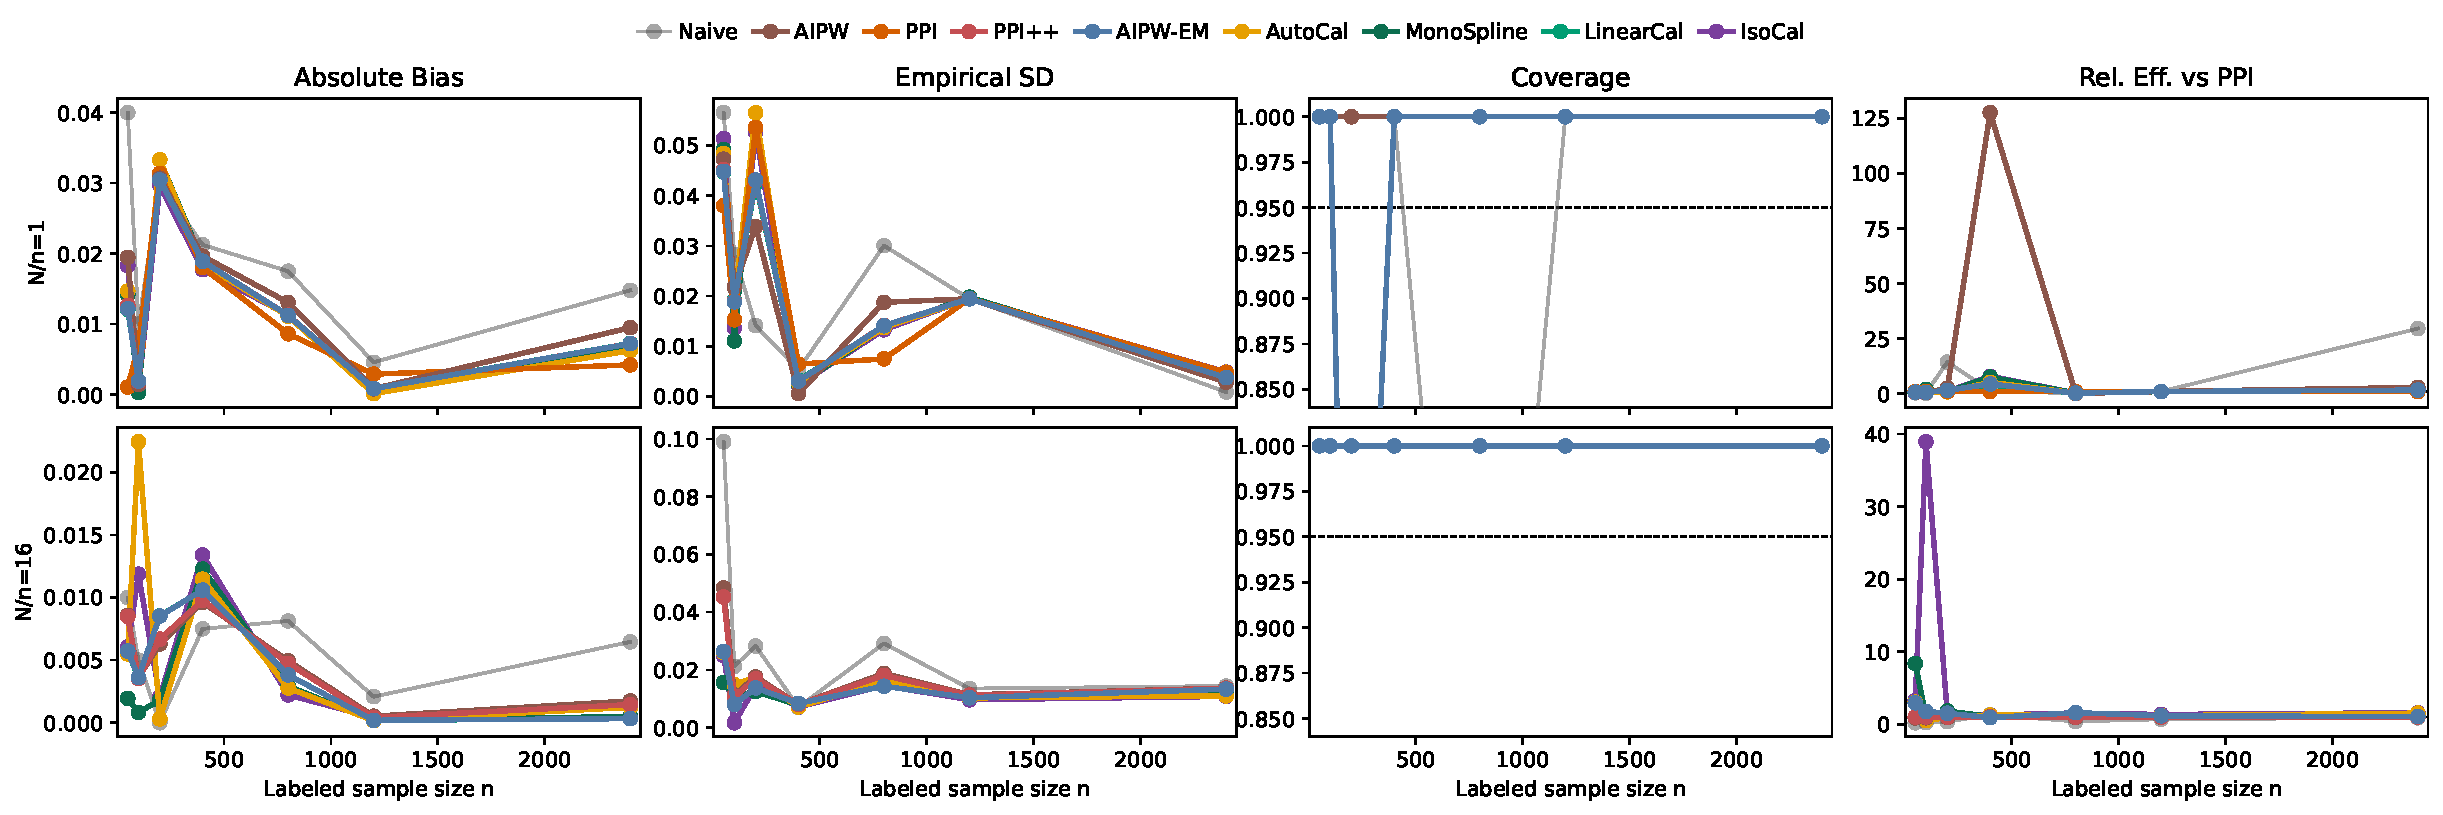
\includegraphics[width=\textwidth]{assets/sim_fig_main.pdf}
\caption{Synthetic simulation study with a poorly calibrated score. The top row shows \(N/n=1\), the bottom row shows \(N/n=16\). Columns report Monte Carlo standard deviation, coverage, and relative efficiency versus PPI.}
\label{fig:simulation-rmse}
\end{figure}

\Cref{fig:simulation-rmse} shows the mechanism directly. The score-based AIPW estimators are essentially unbiased and maintain near-nominal coverage, so the practical distinction is efficiency. AIPW improves on PPI among the raw-score methods, and calibration gives the largest gains when the unlabeled sample is large enough for score quality to dominate. At \(n=400\) and \(N/n=16\), the calibrated methods reduce RMSE from about \(0.0172\) for PPI to about \(0.0164\). The PPI++ comparison is also informative: unclipped \textsc{AIPW-EM} is nearly indistinguishable from \texttt{LinearCal}, whereas clipped PPI++ can fall back toward PPI when the variance-minimizing rescaling exceeds the clipping range.

\paragraph{Reproduced PPI benchmarks} We next evaluate the same idea on the standard PPI mean-estimation benchmarks of \cite{ppi2023},
where any score miscalibration is present in the public score rather than
introduced by design. Using the public \texttt{ppi\_py} \texttt{forest},
\texttt{galaxies}, and \texttt{census\_income} datasets, we rerandomize the
labeled/unlabeled split 500 times at each labeled-sample size and evaluate all
estimators on the same splits.

AIPW is usually the strongest raw-score baseline; PPI is competitive mainly
when the unlabeled sample is extremely large. Calibration gains are therefore
not uniform. On \texttt{forest} and \texttt{galaxies}, the leading score-based
methods are tightly clustered. On \texttt{census\_income}, the score is
sufficiently mis-scaled that \texttt{LinearCal} has the lowest average MSE. The
efficiency-maximization comparison also matches the theory: across the 30
dataset-size cells in the 500-split refresh, unclipped \textsc{AIPW-EM} has
lower MSE than clipped PPI++ in 29 cells and is nearly tied with
\texttt{LinearCal}. This indicates that much of the observed PPI++ gap is due
to clipping rather than empirical efficiency maximization itself.
Appendix~\ref{app:empirical} gives the dataset-by-regime tables and the full
calibration comparison.

\paragraph{LLM evaluation benchmark}  The final experiment studies modern LLM evaluation, where proxy-score miscalibration is common and raw reward-model margins can be badly scaled. The first track uses PPE Human Preference V1 \citep{frick2025evaluate}; the second uses a PPE correctness suite built from MMLU-Pro, MATH, GPQA, IFEval, and MBPP+ \citep{frick2025evaluate,wang2024mmlupro,hendrycksmath2021,rein2024gpqa,zhou2023instructionfollowing,liu2023evalplus}. We use four public precomputed evaluator-score sources on the PPE tracks: Skywork-Reward-Llama-3.1-8B, ArmoRM-Llama3-8B-v0.1, Athene-RM-8B, and Starling-RM-7B-alpha. The final run completed all 112 evaluator/benchmark/target stages, and the reported summaries use 200 rerandomized labeled/unlabeled splits per stage.

The raw proxy can be unsafe as a variance-reduction device even though it contains useful signal. On PPE Human at \(n=100\), raw PPI and raw AIPW have MSE \(0.495\) and \(0.440\), compared with \(0.001425\) for labeled-only and \(0.001391\) for \texttt{LinearCal}. On PPE Correctness at \(n=100\), the corresponding MSEs are \(0.534\), \(0.353\), \(0.002010\), and \(0.001813\). Calibration therefore recovers the stability of labeled-only estimation while still extracting modest label savings from the proxy scores: about \(3\%\) on PPE Human and \(10\%\) on PPE Correctness at \(n=100\). \texttt{LinearCal} is the strongest and most stable method overall, with \texttt{AutoCal} close behind. \Cref{tab:llm-summary-main} in Appendix \ref{app:simresults} summarizes the main PPE numbers, and Appendices \ref{app:llm-eval-by-evaluator} and \ref{app:llm-ranking} give evaluator-specific and ranking-task diagnostics.

\section{Conclusion}

Prediction-powered inference can be viewed as using black-box predictions as
AIPW regression adjustments. These adjustments improve efficiency to the extent
that they approximate the target outcome regression. Post-hoc calibration offers
a simple way to improve this approximation without retraining the predictor,
while preserving AIPW-style validity. This perspective clarifies several existing PPI procedures. In particular,
PPI++ is first-order equivalent to linear calibration, while isotonic
calibration provides a nonlinear score-only adjustment with valid inference and
first-order optimality among monotone transformations. Empirically, raw proxy
scores can be poorly scaled, especially in LLM evaluation settings; calibration
often recovers labeled-only stability and can improve efficiency when the score
contains useful ranking information. Overall, calibration provides a principled post-hoc route for turning an
informative but miscalibrated score into a more effective regression adjustment
for prediction-powered inference.

\bibliographystyle{plainnat}
\bibliography{references}

\appendix

\section{LLM simulation results}
\label{app:simresults}
\IfFileExists{assets/table_llm_summary.tex}{
\begin{table}[h]
\centering
\small
\resizebox{\textwidth}{!}{\begin{tabular}{lllrccc}
\toprule
Track & $n$ & Estimator & MSE / PPI & RelEff / PPI & Coverage & Label savings \\
\midrule
PPE Correctness & 25 & AIPW & 0.878 & 1.367 & 0.850 & 0.113 \\
PPE Correctness & 25 & AIPW-EM & 0.520 & 1157.062 & 0.844 & 0.202 \\
PPE Correctness & 25 & AutoCal & 0.524 & 1515.978 & 0.856 & 0.210 \\
PPE Correctness & 25 & Labeled-only & 0.500 & inf & 0.900 & 0.000 \\
PPE Correctness & 25 & IsoCal & 0.452 & 11575.686 & 0.875 & 0.194 \\
PPE Correctness & 25 & LinearCal & 0.501 & 7335.829 & 0.850 & 0.208 \\
PPE Correctness & 25 & MonoSpline & 0.481 & 1041.054 & 0.844 & 0.228 \\
PPE Correctness & 25 & Platt & 0.498 & 12288.149 & 0.863 & 0.241 \\
PPE Correctness & 25 & PPI & 1.000 & 1.000 & 0.850 & 0.110 \\
PPE Correctness & 25 & PPI++ & 0.473 & inf & 0.850 & 0.132 \\
PPE Correctness & 50 & AIPW & 0.751 & 1.769 & 0.931 & 0.112 \\
PPE Correctness & 50 & AIPW-EM & 0.429 & 6018.106 & 0.938 & 0.220 \\
PPE Correctness & 50 & AutoCal & 0.383 & 6184.299 & 0.931 & 0.205 \\
PPE Correctness & 50 & Labeled-only & 0.376 & inf & 0.950 & 0.000 \\
PPE Correctness & 50 & IsoCal & 0.408 & inf & 0.925 & 0.240 \\
PPE Correctness & 50 & LinearCal & 0.438 & 4487.608 & 0.938 & 0.217 \\
PPE Correctness & 50 & MonoSpline & 0.425 & 148597065531295156473430016.000 & 0.919 & 0.239 \\
PPE Correctness & 50 & Platt & 0.426 & 7455.383 & 0.931 & 0.225 \\
PPE Correctness & 50 & PPI & 1.000 & 1.000 & 0.938 & 0.102 \\
PPE Correctness & 50 & PPI++ & 0.345 & inf & 0.938 & 0.192 \\
PPE Human Preference & 25 & AIPW & 0.832 & 2.390 & 0.938 & 0.141 \\
PPE Human Preference & 25 & AIPW-EM & 0.340 & 489.182 & 1.000 & 0.177 \\
PPE Human Preference & 25 & AutoCal & 0.378 & 488.899 & 1.000 & 0.176 \\
PPE Human Preference & 25 & Labeled-only & 0.464 & 545.093 & 1.000 & 0.000 \\
PPE Human Preference & 25 & IsoCal & 0.369 & 427.847 & 1.000 & 0.172 \\
PPE Human Preference & 25 & LinearCal & 0.345 & 495.939 & 1.000 & 0.173 \\
PPE Human Preference & 25 & MonoSpline & 0.338 & 293.144 & 1.000 & 0.228 \\
PPE Human Preference & 25 & PPI & 1.000 & 1.000 & 0.938 & 0.140 \\
PPE Human Preference & 25 & PPI++ & 0.376 & 461.364 & 1.000 & 0.145 \\
PPE Human Preference & 50 & AIPW & 0.751 & 1.378 & 1.000 & 0.010 \\
PPE Human Preference & 50 & AIPW-EM & 0.338 & 136.356 & 1.000 & 0.138 \\
PPE Human Preference & 50 & AutoCal & 0.329 & 161.658 & 1.000 & 0.148 \\
PPE Human Preference & 50 & Labeled-only & 0.265 & 172.214 & 1.000 & 0.000 \\
PPE Human Preference & 50 & IsoCal & 0.446 & 152.657 & 1.000 & 0.087 \\
PPE Human Preference & 50 & LinearCal & 0.335 & 138.599 & 1.000 & 0.140 \\
PPE Human Preference & 50 & MonoSpline & 0.350 & 153.849 & 1.000 & 0.042 \\
PPE Human Preference & 50 & PPI & 1.000 & 1.000 & 1.000 & 0.012 \\
PPE Human Preference & 50 & PPI++ & 0.280 & 104.304 & 1.000 & 0.037 \\
\bottomrule
\end{tabular}
}
\caption{PPE LLM-evaluation summary at \(n\in\{100,400\}\), macro-averaged across the public evaluator models. MSE/PPI reports MSE normalized to raw PPI; label savings is relative to labeled-only; coverage is Wald-interval coverage.}
\label{tab:llm-summary-main}
\end{table}
}{}

\section*{Appendix Contents}
The appendix is ordered from background and practical guidance to extensions, proofs, empirical details, and the anonymous implementation sketch.
\begin{enumerate}[leftmargin=7mm,label=\Alph*.]
\item \hyperref[app:related-work]{Extended related work}
\item \hyperref[app:semicolon]{Semiparametric background}
\item \hyperref[appendix:remarks]{Additional remarks}
\item \hyperref[app:causal]{Calibrated DML for randomized trials}
\item \hyperref[appendix::momentgeneral]{Moment equations under missing at random}
\item \hyperref[app:iid]{Pooled i.i.d. missing-data formulation}
\item \hyperref[app:repr]{Proof of the representation theorem}
\item \hyperref[sec:ppi++]{PPI++ and linear calibration}
\item \hyperref[app:eif]{Proof of the AIPW influence-pair characterization}
\item \hyperref[app:iso-lemmas]{Supporting lemmas for calibration}
\item \hyperref[app:al]{Proof of asymptotic linearity}
\item \hyperref[app:eff]{Proof of post-processing equivalence and reduced-model efficiency}
\item \hyperref[app:empirical]{Additional empirical details}
\item \hyperref[appendix:code]{Anonymous implementation sketch}
\end{enumerate}

\section{Extended related work}
\label{app:related-work}

Although PPI is often presented as a recent development, the underlying estimation problem and many of its estimators are special cases of a broader literature on semiparametric debiasing and regression adjustment, including work on missing data, causal inference, and debiased machine learning.

\textbf{Semiparametric statistics and missing data.} Our problem sits squarely in the missing-data and semiparametric literatures. \citet{rubin1976} formalized missing at random as a key identification condition for recovering full-data targets from partially observed outcomes. Semiparametric efficiency theory then characterized efficient influence functions, regular asymptotically linear estimators, and one-step debiased procedures \citep{levit1975efficiency,pfanzagl1985contributions,hasminskii1979nonparametric,klaassen1987consistent,bickel1993efficient}. In missing-data and causal-inference problems, these ideas led to influence-function-based estimating equations \citep{robins1994estimation,robins1995analysis,robins1995semiparametric,vanderlaanunified,tsiatis2006semiparametric}, often with doubly robust structure \citep{bang2005doubly}. Accordingly, the efficiency theory for missing-data models under missingness or coarsening at random is well understood, and the class of regular asymptotically linear estimators in these models can be characterized through their influence functions \citep{robins1994estimation,robins1995analysis,robins1995semiparametric,vanderlaanunified,tsiatis2006semiparametric}.

\textbf{Debiased machine learning and targeted learning.} A large body of work combines the semiparametric framework above with machine-learning-based nuisance estimation, often under the label of debiased machine learning. Flexible learning methods within estimating equations and AIPW-style procedures already appear in \citet{vanderlaanunified}. Targeted minimum loss estimation (TMLE), or targeted learning, updates an initial nuisance estimator in a parameter-targeted way so that the resulting plug-in estimator is debiased; in the present setting, the main nuisance is the outcome regression \citep{van2006targeted,vanderLaanRose2011,gruber2009targeted,hoffman2020tmle,ross2025constructing}. These approaches are often combined with sample splitting and cross-fitting to accommodate generic machine-learning estimators \citep{schick1986asymptotically,klaassen1987consistent,zheng2010asymptotic,vanderLaanRose2011,DoubleML}. Double machine learning emphasizes similar ingredients---orthogonality, cross-fitting, and influence-function expansions---for inference with modern nuisance estimators \citep{DoubleML,chernozhukov2022automatic}, and can be understood within the same semiparametric framework \citep{vanderlaan2019cvtmle,diaz2020machine,chen2026equivalence}. For sufficiently stable estimators, cross-fitting can itself be relaxed \citep{chen2022stable}. Closely related work studies balancing-weight estimators \citep{hainmueller2012entropy,imai2014covariate,zubizarreta2015stable,lendle2015balancing,chattopadhyay2020balancing,hejazi2023revisiting}, which often admit equivalent regression-adjustment or augmented representations \citep{chattopadhyay2023implied,bruns2025augmented,rotnitzky2025note}. In completely missing-at-random settings, including semisupervised learning and randomized trials, these approaches allow flexible black-box nuisance estimation while still supporting valid inference under appropriate conditions \citep{moore2009covariate,moore2009increasing,rosenblum2009using,hojbjerre2025powering,hojbjerre2026within}.

\textbf{Semisupervised inference.} Related work studies semisupervised or surrogate-assisted estimation in settings where the primary outcome is observed only on a limited subset, while auxiliary outcomes or surrogate measurements are available more broadly \citep{pepe1992inference,pepe1994auxiliary,chen2000miscellanea,chen2008improving,cheng2021robust,ji2025predictions,kallus2025role}. Two-sample semisupervised inference is a special case of two-stage sampling designs \citep{scott1982effect,rose2011targeted,hejazi2021efficient,qiu2026efficient} and, more generally, of data fusion, for which a substantial semiparametric efficiency literature has been developed \citep{li2023efficient,li2025data,graham2024towards,xu2025unified}. More recent papers have used the term \emph{prediction-powered inference} (PPI) for the semisupervised mean-estimation setting in which a black-box predictor is combined with a small labeled sample and a large unlabeled sample \citep{ppi2023,angelopoulos2023ppi,crossppi2024,xu2025unified,song2026demystifying,poulet2025prediction,lee2026mec}. These papers also helped popularize such methods for a broader machine-learning audience and provided accessible software. Closely related questions have long been studied in randomized trials, where prognostic scores or other regression adjustments learned from larger historical or auxiliary data sources are used to improve precision in smaller trials \citep{hansen2008prognostic,rosenblum2009using,moore2009covariate,moore2009increasing,moore2011robust,schuler2022increasing,balzer2024adaptive,hojbjerre2025powering}. Methodologically, however, PPI estimators are best understood as instances or variants of existing semiparametric procedures. For example, PPI++ is an AIPW estimator \citep{robins1994estimation,vanderlaanunified} obtained by empirical efficiency maximization \citep{rubin2008empirical} over a scaling parameter, and cross-PPI \citep{crossppi2024} is simply AIPW with cross-fitting. MEC \citep{lee2026mec} instead uses generalized entropy weights to balance the prediction score, which is closer to the balancing-weight representation of our linearly calibrated estimator. Our linearly calibrated estimator emphasizes the corresponding regression-adjustment view, implemented by ordinary linear regression of \(Y\) on the score. More fundamentally, the ability to combine black-box prediction models with valid inference is a consequence of the double robustness of AIPW when the missingness probability is known, and is not specific to semisupervised mean estimation \citep{bang2005doubly,seaman2018introduction,rotnitzky2021characterization}.

\textbf{From missing data to causal inference.} From the perspective of estimation and efficiency theory, semisupervised mean estimation with missing-at-random outcomes is equivalent to randomized experiments, controlled trials, and survey-sampling designs once the missingness indicator is reinterpreted as a treatment or sampling indicator, so that the relevant potential outcomes are viewed as missing \citep{rubin1978bayesian,vanderlaanunified,licausal,mozer2026ppi}. This equivalence allows tools from covariate adjustment, causal inference, and model-assisted estimation to be transferred directly to the semisupervised setting; see, for example, \citet{mozer2026ppi} for results relating prediction-powered inference to model-assisted survey-sampling estimators. The two-sample formulation we study is also equivalent to a one-sample i.i.d.\ model \citep{li2023efficient}. In particular, our methods apply to inference on the counterfactual mean \(\mathbb{E}[Y(1)]\) in a randomized trial with binary treatment, where treated units form the labeled sample and control units contribute covariate information only; see Appendix \ref{app:causal}.

\textbf{Calibration.} A final relevant thread concerns calibration. Classical post-processing methods such as Platt scaling \citep{platt1999probabilistic,cox1958two,gupta2023online}, linear calibration \citep{mincer1969evaluation,chernozhukov2018generic,leng2021calibration}, isotonic regression \citep{zadrozny2002transforming,niculescu2005predicting}, and histogram binning \citep{zadrozny2001obtaining,gupta2021distribution} improve predictive reliability without retraining the underlying model. The idea has deeper roots in the forecasting literature \citep{mincer1969evaluation,lichtenstein1977calibration,vovk1992universal,vovk2005algorithmic,gneiting2007probabilistic,lambert2011elicitation}; see also the historical discussion in \citet{lee2023t}. More recent work studies calibration under broader losses and prediction tasks \citep{jung2021moment,noarov2023statistical,van2023causal,whitehouse2024orthogonal,van2025venn}, as well as applications to conformal prediction \citep{van2024self,van2025venn}, importance-weight stabilization \citep{gutman2022propensity,deshpande2023calibrated,ballinari2024improving,van2024stabilized}, treatment effect estimation \citep{chernozhukov2018generic,van2023causal,whitehouse2024orthogonal}, and value prediction in offline reinforcement learning \citep{van2025bellman}. Distribution-free guarantees for histogram binning are developed by \citet{gupta2021distribution}, while \citet{van2023causal,van2025venn} establish asymptotic distribution-free guarantees for isotonic calibration. Most closely related to our work is recent research connecting calibration to debiased estimation of statistical functionals \citep{van2024automatic,van2023adaptive,van2025semiparametric}. In particular, \citet{van2024automatic} studies calibrated debiased machine learning for doubly robust inference, which in our setting reduces to calibrating the outcome regression and exploiting the resulting plug-in representation, while \citet{van2025semiparametric} studies calibrated plug-in regression estimators in reinforcement learning. More broadly, \citet{van2023adaptive} shows how plug-in calibration can support regression and treatment effect estimation, including superefficient inference through dimension reduction.

\section{Semiparametric background}
\label{app:semicolon}

\subsection{Review of AIPW, PPI, and semiparametric efficiency}
\label{sec:effreview}

\textbf{The AIPW class.} We begin with the augmented inverse-probability weighted (AIPW) estimator in the unrestricted two-sample model \citep{robins1994estimation}. We view AIPW not as a single estimator, but as a family of estimators indexed by a regression-adjustment score \(q:\mathcal X\to\R\) with finite second moment. For any such \(q\), define
\begin{equation}
\label{eq:aipw-family}
\widehat\psi(q)
:=
\Pmx q+\Pl\{Y-q(X)\}.
\end{equation}
This estimator combines a plug-in term that imputes \(Y\) from \(q(X)\) with a residual correction from the labeled sample. For any fixed \(q\), \(\widehat\psi(q)\) is unbiased in finite samples for \(\psi_0=\E_{P_0}[Y]\). In particular, \(q(X)=0\) yields the empirical mean estimator \(\mathbb{P}_n^L\{Y\}\). Thus, the choice of \(q\) affects efficiency, through the estimator's variance, but not validity, in the sense that the resulting confidence intervals remain valid. This makes AIPW a ``safe'' estimator \citep{xu2025unified}. This property can be viewed as a particularly simple instance of double robustness\footnote{In more general missing-at-random settings with unknown, covariate-dependent missingness probabilities, the analogous AIPW estimator remains doubly robust asymptotically, but it no longer enjoys the same finite-sample unbiasedness as in the present known-\(\rho_n\) setting \citep{seaman2018introduction}.} \citep{bang2005doubly}. The same basic principle underlies the use of flexible machine learning for covariate adjustment in randomized trials while retaining valid inference \citep{moore2009covariate,moore2009increasing,schuler2022increasing,hojbjerre2025powering}.

\textbf{Asymptotic linearity and efficiency.} To characterize the leading large-sample error in the two-sample model, we decompose the estimation error into one contribution from the labeled sample and one from the unlabeled sample. We say that \(\widehat\psi\) is asymptotically linear with influence pair \((D^L,D^U)\) if
\[
\widehat\psi-\psi_0
=
\frac{1}{M}\sum_{i=1}^n D^L(X_i,Y_i)
+
\frac{1}{M}\sum_{j=1}^N D^U(\widetilde X_j)
+
o_p(M^{-1/2}),
\]
where \(\E_{P_0}[D^L(X,Y)]=0\) and \(\E_{\Px}[D^U(\widetilde X)]=0\). By the central limit theorem and the independence of the two samples,
\[
\sqrt{M}\,(\widehat\psi-\psi_0)
\rightsquigarrow
N\!\left(0,\,
\rhozero \Var_{P_0}\{D^L(X,Y)\}
+
(1-\rhozero)\Var_{\Px}\{D^U(\widetilde X)\}\right).
\]
The influence pair therefore determines the estimator's asymptotic variance and provides a convenient way to compare efficiency across different choices of \(q\). The next result uses this representation to characterize the AIPW class, identify the efficient influence pair in the unrestricted two-sample model, and thereby obtain the semiparametrically efficient variance bound \citep{bickel1993efficient}.

\begin{proposition}[Influence pair for the AIPW class]
\label{prop:aipw-class}
Under \cref{assump:design}, for any fixed \(q:\mathcal X\to\R\) with finite second moment, the estimator \(\widehat\psi(q)\) is asymptotically linear with influence pair \((D_q^L,D_q^U)\), where
\begin{align}
\label{eq:if-class-L}
D_q^L(X,Y)
&=
q^\circ(X)-\psi_0+\rhozero^{-1}\{Y-q^\circ(X)\},\\
\label{eq:if-class-U}
D_q^U(\widetilde X)
&=
q^\circ(\widetilde X)-\psi_0,
\end{align}
with \(q^\circ(X):=q(X)-\E_{\Px}\{q(X)\}+\psi_0\)
denoting the recentered version of \(q(X)\). The resulting asymptotic variance of \(\sqrt{M}\,(\widehat\psi(q)-\psi_0)\) is
\begin{align*}
\Var\{\mu_0(X)\}
+
\rho_0^{-1}\E_{P_0}\!\bigl[\Var(Y\mid X)\bigr]
+
\frac{1-\rho_0}{\rho_0}\E_{P_0}\!\bigl[(q^\circ(X)-\mu_0(X))^2\bigr].
\end{align*}
This variance is minimized over the AIPW class when \(q^\circ=\mu_0\), in particular at \(q=\mu_0\). Therefore, the efficient influence pair for \(\psi_0=\E_{P_0}[Y]\) in the unrestricted two-sample model is \((D_{\mu_0}^L,D_{\mu_0}^U)\), and the corresponding asymptotic variance is the efficiency bound \citep{robins1995analysis,robins1995semiparametric,tsiatis2006semiparametric}.
\end{proposition}

A key insight of Proposition~\ref{prop:aipw-class} is that the limiting variance of the AIPW estimator depends on the score function \(q\) only through the mean squared error of its recentered version \(q^\circ\), namely \(\E_{P_0}\!\bigl[(q^\circ(X)-\mu_0(X))^2\bigr]\). Thus, within the AIPW class, efficiency is maximized by choosing \(q\) so that \(q^\circ\) approximates \(\mu_0(X)\) as well as possible, with equality when \(q^\circ=\mu_0\), in particular at \(q=\mu_0\). This shows that full efficiency generally requires using the full covariate information \(X\), or at least a summary rich enough to recover \(\mu_0(X)\) \citep{robins1995semiparametric}. In practice, this motivates taking \(q\) to be an estimated prediction score \(m(X)\), learned using flexible black-box methods.

\textbf{AIPW, PPI, and empirical-efficiency maximization.}
We now record several familiar choices of \(q\) within the class \eqref{eq:aipw-family}. The most common choice is \(q(X)=m(X)\), where \(m(X)\) is a prediction score, yielding the usual augmented inverse-probability weighted (AIPW) estimator \citep{robins1994estimation}:
\[
\widehat{\psi}_{\mathrm{AIPW}}
=
\rhon \Pl\{m(X)\}
+
(1-\rhon)\Pu\{m(\widetilde X)\}
+
\Pl\{Y-m(X)\}.
\]
Equivalently,
\[
\widehat{\psi}_{\mathrm{AIPW}}
=
\frac{1}{M}\left\{
\sum_{i=1}^n m(X_i)
+
\sum_{j=1}^N m(\widetilde X_j)
+
\frac{1}{\rho_n}\sum_{i=1}^n \{Y_i-m(X_i)\}
\right\},
\]
where \(\rho_n^{-1}\) is the inverse probability of observing the outcome.

Another estimator in this class was considered by \citet{ppi2023} under the name PPI,\footnote{The PPI and PPI++ estimators are algebraically equivalent to the model-assisted survey-design estimators of \citet{cassel1976some} and \citet{sarndal2003model}, respectively; see \citet{mozer2026ppi} for a review.} and we adopt that terminology here. It corresponds to the score choice
\[
q(X)=\frac{m(X)}{1-\rho_n}.
\]
Substituting this choice into \eqref{eq:aipw-family} gives
\[
\widehat{\psi}_{\mathrm{PPI}}
=
\Pu\{m(\widetilde X)\}+\Pl\{Y-m(X)\}.
\]
Relative to \(\widehat{\psi}_{\mathrm{AIPW}}\), \(\widehat{\psi}_{\mathrm{PPI}}\) uses only the unlabeled sample in the plug-in term and rescales the score by the factor \((1-\rho_n)^{-1}>1\). By Proposition~\ref{prop:aipw-class}, this helps only if the rescaled score is closer to \(\mu_0(X)\) in mean squared error. Thus, PPI is inefficient when \(m=\mu_0\), and is typically less efficient when \(m\) is already reasonably accurate. When \(\rho_n\) is small and \(m\) is sufficiently inaccurate, however, neither estimator is necessarily more efficient than the other \citep{han2012note,rotnitzky2012improved}.

Because both \(\widehat{\psi}_{\mathrm{AIPW}}\) and \(\widehat{\psi}_{\mathrm{PPI}}\) use scores in the scaling class \(\{\lambda m(X):\lambda\in\mathbb R\}\), one can choose the scaling factor data-adaptively rather than fixing it in advance. One way to do so is to minimize an empirical estimate of the asymptotic
variance of \(\sqrt M\{\widehat\psi(q)-\psi_0\}\):
\[
\sigma_n^2(q):=
\rho_n\,\widehat{\operatorname{Var}}_L
\{q(X)+\rho_n^{-1}(Y-q(X))\}
+(1-\rho_n)\,\widehat{\operatorname{Var}}_U\{q(\widetilde X)\},
\]
where \(\widehat{\operatorname{Var}}_L(a):=\Pl[(a-\Pl a)^2]\) and
\(\widehat{\operatorname{Var}}_U(b):=\Pu[(b-\Pu b)^2]\).
That is, one chooses \(\lambda\) to minimize \(\sigma_n^2(q)\) over \(q(X)=\lambda m(X)\), a procedure known as empirical-efficiency maximization \citep{rubin2008empirical,vanderlaanunified}. The resulting estimator, called PPI++ by \citet{angelopoulos2023ppi}, is simply the AIPW estimator with an empirically rescaled prediction rule \(\hat\lambda m(X)\), where \(\hat\lambda\) estimates the population-optimal scaling coefficient
\begin{equation}
\label{opt:scale-app}
\lambda^\star
=
\frac{\Cov\bigl(Y,m(X)\bigr)}{\Var\bigl(m(X)\bigr)}.
\end{equation}
The same principle extends beyond simple rescaling. For example, one can minimize \(\sigma_n^2(q)\) over richer classes such as $\{\lambda m(X)+\beta_{\mathrm{lin}}^\top X:
\lambda \in \mathbb R,\ \beta_{\mathrm{lin}} \in \mathbb R^d\},$
over monotone transformations of the score, or over a reproducing kernel Hilbert space (Appendix \ref{appendix:remarks}). More generally, the same criterion can be used in cross-validation to choose among candidate estimator classes \citep{rubin2008empirical}.

Regression adjustment and TMLE can yield the efficient influence pair by
updating the regression so that its empirical residual mean vanishes
\citep{scharfstein1999adjusting,van2006targeted,rosenblum2009using}.
The calibration identity \eqref{eqn::aipwcal} gives an exact instance of this construction.

\section{Additional remarks}

\label{appendix:remarks}

\begin{remark}[Implementation]
Isotonic regression is widely available in standard software. A standard algorithm is the pooled-adjacent-violators algorithm (PAVA) \citep{barlow1972isotonic}. Although it is generally fast, it may become slow at ultra-large sample sizes. A scalable alternative is to use regression tree software with monotonicity constraints, such as XGBoost or LightGBM (see Appendix \ref{appendix:code}). An advantage of tree-based software is that the fit can be regularized by constraining or tuning the number of leaves, the maximum tree depth, or the minimum number of observations per leaf.
\end{remark}

\begin{remark}[Platt scaling adjustment]
The linear-calibration idea extends beyond squared-error loss. One can instead use logistic loss, Poisson loss, or, more generally, losses from canonical-link generalized linear models \citep{rosenblum2009using}. In particular, when \(Y\in\{0,1\}\) and \(\mhat(X)\in(0,1)\) is an initial predictor, one may apply Platt scaling \citep{cox1958two,platt1999probabilistic} by fitting a logistic regression of \(Y\) on the logit of \(\mhat(X)\). Writing \(\eta_i(a,b):=a\,\mathrm{logit}(\mhat(X_i))+b\), this amounts to solving
\begin{equation}
\label{eq:platt-cal}
\begin{split}
\bigl(\hat a_{\mathrm{platt}},\hat b_{\mathrm{platt}}\bigr)
\in
\arg\min_{a,b\in\R}
\sum_{i=1}^n
\Bigl[
 -Y_i \log \sigma\bigl(\eta_i(a,b)\bigr) \\
 \qquad\qquad
 -(1-Y_i)\log\Bigl(1-\sigma\bigl(\eta_i(a,b)\bigr)\Bigr)
\Bigr].
\end{split}
\end{equation}
with calibrated predictor
\[
q_n^{\mathrm{platt}}(X)
:=
\sigma\bigl(\hat a_{\mathrm{platt}}\,\mathrm{logit}(\mhat(X))+\hat b_{\mathrm{platt}}\bigr),
\]
where \(\sigma(t):=(1+e^{-t})^{-1}\). Platt scaling may be preferred over linear regression calibration when predicted probabilities are systematically over- or under-confident, in which case the calibration curve is often approximately sigmoidal. More generally, outcomes can be rescaled to \([0,1]\) before applying this procedure. In online settings, calibration properties of Platt scaling are developed in \cite{gupta2023online}.
\end{remark}

\subsection{Cross-Fitting and Cross-Calibration}
\label{sec:crossfit}

In the main exposition, we assume for simplicity that the initial black-box predictor is fixed. In practice, however, it may be trained on the labeled sample itself, in which case the same labeled observations are used both to fit the predictor and to calibrate its scores. A cross-fitted version avoids this reuse by replacing the single prediction function with out-of-fold predictions and then fitting the calibrator to the resulting labeled out-of-fold scores.

\begin{enumerate}[leftmargin=6mm,label=\arabic*.]
\item Partition the labeled sample indices into folds \(I_1,\dots,I_K\).
\item For each fold \(k\), train the black-box regression \(\mhat^{(-k)}\) on the labeled observations outside \(I_k\), compute out-of-fold predictions \(\mhat^{(-k)}(X_i)\) for \(i\in I_k\), and compute predictions \(\mhat^{(-k)}(\widetilde X_j)\) on the unlabeled sample.
\item Pool the labeled out-of-fold predictions \(\{\mhat^{(-k(i))}(X_i)\}_{i=1}^n\) and fit a calibrator \(\fhat\) to the labeled pairs \((\mhat^{(-k(i))}(X_i),Y_i)\).
\item Form calibrated predictions
\[
\mtilde(X_i)=\fhat(\mhat^{(-k(i))}(X_i))
\]
and
\[
\mtilde(\widetilde X_j)=\frac{1}{K}\sum_{k=1}^K \fhat(\mhat^{(-k)}(\widetilde X_j)),
\]
and then compute the plug-in estimator in \cref{eq:plugin}.
\end{enumerate}

This cross-fitted modification is the natural DML-style implementation when one wishes to reduce overfitting from using the same labeled data both to estimate the initial regression and to calibrate it for inference \citep{zheng2010asymptotic,vanderLaanRose2011,DoubleML}. Related procedures have been used for debiased inference in \citet{van2024stabilized,van2024automatic,rabenseifner2025causal}, and a related cross-calibration variant appears in \citet{van2023causal}.

\begin{remark}[Empirical efficiency maximization over a prediction class]
The empirical variance criterion \(\sigma_n^2(q)\) in Section~\ref{sec:effreview}
can be minimized over any candidate class \(\mathcal G\subset L^2(\Px)\):
\[
\hat q\in\arg\min_{q\in\mathcal G}\sigma_n^2(q),
\qquad \widehat\psi_{\mathrm{eem}}:=\widehat\psi(\hat q).
\]
For a fixed score, Proposition~\ref{prop:aipw-class} gives the population criterion
\[
V(q)=\Var(Y)+\frac{1-\rhozero}{\rhozero}\Var\{Y-q(X)\}.
\]
Writing \(q^\circ=q-\E_{\Px}q+\psi_0\), we have
\(\Var\{Y-q(X)\}=\E[(Y-q^\circ(X))^2]\).
If \(\mathcal G\) is closed under constant shifts, population least-squares
regression therefore targets a variance-minimizing score.
For tuning, average held-out estimates of the influence-function variance
across folds and use the selected class or tuning parameter in a cross-fitted
AIPW estimator \citep{rubin2008empirical}.
\end{remark}

\begin{remark}[Shrinkage via Venn--Abers]
When the labeled sample is small, isotonic calibration may be unstable. A natural alternative is Venn--Abers calibration, originally introduced for binary classification \citep{vovk2012venn}; see \cite{van2024self, van2025venn} for generalized versions beyond the binary setting. Assume \(Y \in [0,1]\), or rescale otherwise. For each \(x\), augment the labeled calibration sample with the hypothetical point \((\mhat(x),y)\) for \(y \in \{0,1\}\), fit the resulting isotonic calibrators \(f_n^{(x,0)}\) and \(f_n^{(x,1)}\), and form the interval-valued prediction
\[
\bigl[f_n^{(x,0)}\{\mhat(x)\},\, f_n^{(x,1)}\{\mhat(x)\}\bigr].
\]
For the Venn--Abers comparator, we shrink the interval midpoint toward the unadjusted AIPW estimator:
\[
q_n^{\mathrm{VA}}(x)
:=
q_n^{\mathrm{mid}}(x)
+
\bigl\{f_n^{(x,1)}\{\mhat(x)\}-f_n^{(x,0)}\{\mhat(x)\}\bigr\}
\bigl\{\widehat\psi_{AIPW}-q_n^{\mathrm{mid}}(x)\bigr\},
\]
where
\[
\begin{aligned}
q_n^{\mathrm{mid}}(x)
&:=
\frac{f_n^{(x,1)}\{\mhat(x)\}+f_n^{(x,0)}\{\mhat(x)\}}{2}.
\end{aligned}
\]
The shrinkage weight is the width of the Venn--Abers interval.
\end{remark}

\begin{remark}[Intercept-only calibration]
Set \(\hat a_{\mathrm{const}}:=\Pl\{Y-\mhat(X)\}\) and
\(q_n^{\mathrm{const}}:=\mhat+\hat a_{\mathrm{const}}\).
Then PPI is the unlabeled mean \(\Pu q_n^{\mathrm{const}}\), whereas
AIPW is the pooled mean \(\Pmx q_n^{\mathrm{const}}\).
\end{remark}

\section{Calibrated DML for randomized trials}
\label{app:causal}

Let \(A\in\{0,1\}\) denote randomized treatment and
\(Y=AY(1)+(1-A)Y(0)\). Assume consistency, no interference, and
\(A\perp(X,Y(1),Y(0))\), with positive assignment probabilities.
For each arm \(a\), the other arm supplies unlabeled covariates when
estimating \(\mu_a:=\E[Y(a)]\).
Let \(\mathbb P_{n,a}\) denote the empirical mean in arm \(a\),
\(\mathbb P_n\) the pooled mean, and \(\hat\pi_a=n_a/n\).
If the calibrated arm-specific score satisfies
\(\mathbb P_{n,a}\{Y-m_{n,a}^\star(X)\}=0\), then
\begin{align}
\hat\mu_a^{\mathrm{cal}}
&:=\mathbb P_n\{m_{n,a}^\star(X)\}\label{eq:rct-mua-plugin}\\
&=\mathbb P_n\{m_{n,a}^\star(X)\}
+\mathbb P_n\left[
\frac{\1(A=a)}{\hat\pi_a}\{Y-m_{n,a}^\star(X)\}
\right].\label{eq:rct-mua-aipw}
\end{align}
The residual correction is zero because it equals
\(\mathbb P_{n,a}\{Y-m_{n,a}^\star(X)\}\).
Thus \eqref{eqn::aipwcal} applies to each arm, and the calibrated
treatment-effect estimator is
\begin{equation}
\label{eq:rct-ate}
\hat\tau^{\mathrm{cal}}:=\hat\mu_1^{\mathrm{cal}}-\hat\mu_0^{\mathrm{cal}}.
\end{equation}
These arm-specific updates are instances of calibrated DML
\citep{van2024automatic}.

\section{Moment equations under missing at random}
\label{appendix::momentgeneral}
For a target satisfying \(\E[\phi_{\theta_0}(X,Y)]=0\), let
\(R\) indicate an observed outcome, \(\pi_0(X)=\Pr(R=1\mid X)>0\), and
\(a_\theta(X)=\E[\phi_\theta(X,Y)\mid X]\).
Under \(R\perp Y\mid X\), the augmented moment equation is
\[
\mathbb P_M\left[
a_\theta(X)+\frac R{\pi_0(X)}\{\phi_\theta(X,Y)-a_\theta(X)\}
\right]=0.
\]
If calibration makes the empirical residual term vanish, this equation reduces
to \(\mathbb P_M a_\theta=0\). Extensions with estimated missingness probabilities
are studied in \citet{robins1994estimation,robins1995analysis,van2024automatic}.

\section{Pooled i.i.d.\ Missing-Data Formulation}
\label{app:iid}

The joint two-sample setup can be embedded into a pooled i.i.d.\ model by introducing a sample-membership indicator \(R \in \{0,1\}\), where \(R=1\) denotes labeled observations and \(R=0\) denotes unlabeled observations. In that formulation one observes i.i.d.\ data \(O=(X,R,RY)\) with \(\Prob(R=1)=\rhozero\), and the calibrated estimator becomes
\[
\psihat = \mathbb P_M(\mtilde) + \mathbb P_M\left[\frac{R}{\rhozero}\{Y-\mtilde\}\right]
\]
up to the same calibration identity as in the main text. The corresponding observed-data efficient influence function is
\[
q_0(X)-\psi_0+\frac{R}{\rhozero}\{Y-q_0(X)\},
\]
which is the single-sample analogue of the efficient influence pair obtained by applying \cref{prop:aipw-class} to the reduced model with scalar covariate \(\mhat(X)\). Thus the usual i.i.d.\ missing-data formulation is a convenient special case, but the main text keeps the two-dataset structure explicit.

\section{Proof of the representation theorem}
\label{app:repr}

\begin{lemma}[AIPW comparison identity]
\label{lem:aipw-comparison}
Suppose \(\Pl\{Y-q_n(X)\}=0\). For any comparison score \(g\) with finite
empirical averages,
\[
\psihat=\widehat\psi(g)+(1-\rhon)(\Pu-\Pl)(q_n-g).
\]
\end{lemma}
\begin{proof}
The residual equation gives \(\psihat=\widehat\psi(q_n)\).
Subtracting \(\widehat\psi(g)\) and collecting terms proves the identity.
\end{proof}

\begin{proof}[Proof of Theorem~\ref{thm:repr}]
Taking the constant score in \eqref{eq:cal-score} gives
\(\Pl\{Y-q_n(X)\}=0\).
Apply Lemma~\ref{lem:aipw-comparison} with \(g=q_{0,\mathcal F}^\dagger\).
\end{proof}

\section{PPI++ and linear calibration}
\label{sec:ppi++}

\begin{proof}[Proof of Proposition~\ref{prop:ppi++-linear}]
Write
\[
\hat v_L:=\Pl[(m-\Pl m)^2],\quad
\hat v_U:=\Pu[(m-\Pu m)^2],\quad
\hat c_L:=\Pl[(Y-\Pl Y)(m-\Pl m)].
\]
On the event \(\hat v_L>0\), the least-squares normal equations give
\[
\hat a_{\mathrm{lin}}=\frac{\hat c_L}{\hat v_L},
\qquad
\hat b_{\mathrm{lin}}=\Pl Y-\hat a_{\mathrm{lin}}\Pl m.
\]
Differentiating the empirical variance criterion in Section~\ref{sec:effreview} gives
\[
\hat\lambda_{++}
=\frac{\hat c_L}{(1-\rhon)\hat v_L+\rhon\hat v_U}.
\]
Finite second moments and \(\Var[m(X)]>0\) imply
\(\hat v_L,\hat v_U\to_p\Var[m(X)]\) and
\(\hat c_L\to_p\Cov(Y,m(X))\).
Thus \(\Pr(\hat v_L>0)\to1\), both coefficients converge to
\(a_0:=\Cov(Y,m(X))/\Var[m(X)]\), and
\(\hat\lambda_{++}-\hat a_{\mathrm{lin}}=o_p(1)\).

For \(\Delta_n:=\Pu m-\Pl m\), substituting the fitted intercept gives
\[
\widehat\psi_{\mathrm{lin}}=\Pl Y+(1-\rhon)\hat a_{\mathrm{lin}}\Delta_n,
\qquad
\widehat\psi_{++}=\Pl Y+(1-\rhon)\hat\lambda_{++}\Delta_n.
\]
Subtracting proves the exact identity in the proposition.
Independence and finite second moments give
\(\Delta_n=O_p(n^{-1/2}+N^{-1/2})\).
Since \(\rhon\to\rhozero\in(0,1)\), both \(n\) and \(N\) are proportional to \(M\), so
\[
\widehat\psi_{++}-\widehat\psi_{\mathrm{lin}}
=(1-\rhon)o_p(1)\Delta_n=o_p(M^{-1/2}).
\]
\end{proof}

\section{Proof of Proposition~\ref{prop:aipw-class}}
\label{app:eif}

\begin{proof}[Proof of Proposition~\ref{prop:aipw-class}]
Adding a constant to \(q\) leaves \(\widehat\psi(q)\) unchanged, so replace
\(q\) by \(q^\circ=q-\E_{\Px}q+\psi_0\).
Centering the empirical means gives
\[
\widehat\psi(q)-\psi_0
=\rhon(\Pl-P_0)D_{q,n}^L+(1-\rhon)(\Pu-\Px)D_q^U,
\]
where \(D_{q,n}^L=q^\circ-\psi_0+\rhon^{-1}(Y-q^\circ)\).
Replacing \(\rhon^{-1}\) by \(\rhozero^{-1}\) changes this expression by
\[
\left(1-\frac{\rhon}{\rhozero}\right)(\Pl-P_0)(Y-q^\circ)
=o_p(M^{-1/2}),
\]
since \(n/M\to\rhozero>0\) and \(Y-q^\circ\) has finite second moment.
This proves the stated influence-pair expansion.

Write \(A=\mu_0-\psi_0\), \(\delta=q^\circ-\mu_0\), and
\(\varepsilon=Y-\mu_0\). Then
\[
D_q^L=A+\rhozero^{-1}\varepsilon+(1-\rhozero^{-1})\delta,
\qquad D_q^U=A+\delta.
\]
Because \(\E[\varepsilon\mid X]=0\), the covariance terms cancel in
\[
\rhozero\Var(D_q^L)+(1-\rhozero)\Var(D_q^U)
=\Var(\mu_0)+\rhozero^{-1}\E[\Var(Y\mid X)]
+\frac{1-\rhozero}{\rhozero}\E[\delta^2].
\]
The choice \(q^\circ=\mu_0\) removes the last term and gives the missing-data
efficiency bound
\citep{robins1995analysis,robins1995semiparametric,tsiatis2006semiparametric}.
\end{proof}

\section{Supporting lemmas for calibration}
\label{app:iso-lemmas}

\begin{lemma}[Blockwise residual orthogonality]
\label{lem:block}
Let \(B_1,\dots,B_J\) be the pooled adjacent violator blocks of the isotonic fit, and let \(q_n^{\mathrm{iso}}(X_i)=c_j\) for \(i \in B_j\). Then
\[
\sum_{i \in B_j}(Y_i-c_j)=0,
\qquad j=1,\dots,J.
\]
Consequently, for every measurable function \(h:\R \to \R\) such that \(h(q_n^{\mathrm{iso}}(X_i))\) is finite for all \(i\),
\[
\sum_{i=1}^n h(q_n^{\mathrm{iso}}(X_i))\{Y_i-q_n^{\mathrm{iso}}(X_i)\}=0.
\]
\end{lemma}

\begin{proof}
The fitted values from isotonic regression are constant on pooled adjacent violator blocks. The KKT conditions imply that residuals sum to zero on each block. Since \(h(q_n^{\mathrm{iso}}(X_i))=h(c_j)\) for all \(i \in B_j\),
\[
\sum_{i=1}^n h(q_n^{\mathrm{iso}}(X_i))\{Y_i-q_n^{\mathrm{iso}}(X_i)\}
=
\sum_{j=1}^J h(c_j)\sum_{i \in B_j}(Y_i-c_j)
=
0.
\]
\end{proof}

\begin{proof}[Proof of \cref{prop:iso-repr}]
Lemma~\ref{lem:block} gives \eqref{eq:orth}.
By definition, the fitted isotonic score minimizes the empirical squared loss
among all nondecreasing transformations of \(\mhat\), proving the risk
comparison. Taking the identity transformation gives the comparison with the
raw score.
\end{proof}

\begin{proof}[Proof of Proposition~\ref{prop:linear}]
The least-squares normal equations give
\(\Pl(Y-q_n^{\mathrm{lin}})=\Pl[\mhat(Y-q_n^{\mathrm{lin}})]=0\).
Since \(q_n^{\mathrm{lin}}\) is affine in \(\mhat\), this also gives
\(\Pl[q_n^{\mathrm{lin}}(Y-q_n^{\mathrm{lin}})]=0\).
Every affine weight \(a+bq_n^{\mathrm{lin}}\) therefore has zero empirical
residual correction. Adding it to \eqref{eq:linear-plugin} proves
\eqref{eq:linear-ppi}.
\end{proof}

\begin{lemma}[Bounded variation after isotonic post-processing]
\label{lem:bv-post}
Suppose \cref{assump:eff-bv} holds. Let \(T:=\mhat(X)\) and \(S_n:=q_n^{\mathrm{iso}}(X)\). Define
\[
\eta(t):=\E_{P_0}[Y\mid T=t],
\qquad
\eta_n(s):=\E_{P_0}[Y\mid S_n=s].
\]
If \(t\mapsto \eta(t)\) has total variation at most \(V\), then, conditional on the labeled sample, the map \(s\mapsto \eta_n(s)\) has total variation at most \(V\). Moreover, \(|\eta_n(s)|\le C_0\) on the support of \(S_n\).
\end{lemma}
\begin{proof}
We adapt the proof of Lemma 6 in \cite{van2023causal}. Let \(S_n=f_n(T)\), where \(f_n\) is the fitted isotonic map. Conditional on the labeled sample, \(f_n\) is nondecreasing and piecewise constant. Hence, for each \(s\) in the support of \(S_n\), there exists an interval \(B_s\subset \mathbb R\) such that
\[
\{S_n=s\}=\{T\in B_s\}.
\]
Therefore
\[
\eta_n(s)
=
\E_{P_0}[Y\mid S_n=s]
=
\E_{P_0}[\eta(T)\mid T\in B_s].
\]

Let \(\eta=\eta^+-\eta^-\) be the Jordan decomposition of \(\eta\), where \(\eta^+\) and \(\eta^-\) are nondecreasing and
\[
\|\eta\|_{TV}=\|\eta^+\|_{TV}+\|\eta^-\|_{TV}\le V.
\]
Then
\[
\eta_n(s)
=
\E_{P_0}[\eta^+(T)\mid T\in B_s]
-
\E_{P_0}[\eta^-(T)\mid T\in B_s].
\]

If \(s_1<s_2\), then monotonicity of \(f_n\) implies every point of \(B_{s_1}\) is no larger than every point of \(B_{s_2}\). Hence the conditional distribution of \(T\mid T\in B_{s_2}\) first-order stochastically dominates that of \(T\mid T\in B_{s_1}\). Therefore, for any nondecreasing function \(g\),
\[
\E_{P_0}[g(T)\mid T\in B_{s_1}]
\le
\E_{P_0}[g(T)\mid T\in B_{s_2}].
\]
Applying this with \(g=\eta^+\) and \(g=\eta^-\), both maps
\[
s\mapsto \E_{P_0}[\eta^+(T)\mid T\in B_s]
\qquad\text{and}\qquad
s\mapsto \E_{P_0}[\eta^-(T)\mid T\in B_s]
\]
are nondecreasing.

Moreover, each of these conditional expectations takes values in the range of the corresponding function, so
\[
\left\|s\mapsto \E_{P_0}[\eta^+(T)\mid T\in B_s]\right\|_{TV}
\le
\|\eta^+\|_{TV},
\qquad
\left\|s\mapsto \E_{P_0}[\eta^-(T)\mid T\in B_s]\right\|_{TV}
\le
\|\eta^-\|_{TV}.
\]
Hence
\[
\|\eta_n\|_{TV}
\le
\|\eta^+\|_{TV}+\|\eta^-\|_{TV}
=
\|\eta\|_{TV}
\le V.
\]

Finally, if \(|\eta(t)|\le C_0\) on the support of \(T\), then
\[
|\eta_n(s)|
=
\left|\E_{P_0}[\eta(T)\mid T\in B_s]\right|
\le C_0
\]
for all \(s\) in the support of \(S_n\).
\end{proof}

\begin{lemma}[The population isotonic projection is centered]
\label{lem:center}
Under \cref{assump:design,assump:isoreg},
\(\E_{\Px}[q_0^{\mathrm{iso}}(X)]=\psi_0\).
\end{lemma}
\begin{proof}
The isotonic class is closed under constant shifts, so
\(c\mapsto\E[(Y-q_0^{\mathrm{iso}}(X)-c)^2]\) is minimized at \(c=0\).
Its derivative there is \(-2\E[Y-q_0^{\mathrm{iso}}(X)]\), giving the stated identity.
\end{proof}

\textbf{Proof convention.} In the following proofs, fix \(\delta>0\). By \(\sup_x |q_n^{\mathrm{iso}}(x)|=O_p(1)\), there exist a deterministic constant \(C=C_\delta\ge C_0\) and \(n_0<\infty\) such that the event
\[
A_{n,C}:=\Bigl\{\sup_x |q_n^{\mathrm{iso}}(x)|\le C\Bigr\}
\]
satisfies \(P_0(A_{n,C})\ge 1-\delta\) for all \(n\ge n_0\). We carry out the deterministic bounded-class arguments on \(A_{n,C}\), where all implicit constants may depend on \(C\) but not on \(n\). Since \(\delta\) is arbitrary, the resulting rates and distributional statements hold unconditionally.

\begin{lemma}[Isotonic \(L^2\) rate]
\label{lem:isorate}
Suppose \cref{assump:design,assump:isoreg} holds. Then
\[
\|q_n^{\mathrm{iso}}-q_0^{\mathrm{iso}}\|_{2,\Px}^2=O_p(n^{-2/3}).
\]
\end{lemma}

\begin{proof}[Proof of \cref{lem:isorate}]

Let \(T:=\mhat(X)\), \(g_0(T):=\E_{P_0}[Y\mid T]\), and
\[
\mathcal M_C:=\{f(T):f\in\mathcal F_{\mathrm{iso}},\ \|f(T)\|_\infty\le C\}.
\]
By \cref{assump:isoreg}, \(g_0(T)\) is bounded by \(C_0\le C\), and on \(A_{n,C}\) we have \(q_n^{\mathrm{iso}}\in\mathcal M_C\). Since clipping any monotone candidate to \([-C,C]\) preserves monotonicity and can only decrease squared risk against \(g_0(T)\), the population isotonic projection \(q_0^{\mathrm{iso}}\) also belongs to \(\mathcal M_C\). For every \(m\in\mathcal M_C\),
\[
\E_{P_0}[(Y-m)^2]
=
\E_{P_0}[(Y-g_0)^2]+\E_{P_0}[(g_0-m)^2],
\]
which shows that \(q_0^{\mathrm{iso}}\) is the \(L^2(P_T)\)-projection of \(g_0\) onto the closed convex set \(\mathcal M_C\).

Now define the centered class
\[
\mathcal F_0:=\{g=m-q_0^{\mathrm{iso}}:\ m\in\mathcal M_C\}.
\]
For \(g\in\mathcal F_0\), let \(\ell_g(Z):=(Y-q_0^{\mathrm{iso}}(X)-g(X))^2-(Y-q_0^{\mathrm{iso}}(X))^2\), where \(Z=(X,Y)\). Since \(q_n^{\mathrm{iso}}\) minimizes the empirical squared risk over \(\mathcal F_{\mathrm{iso}}\), on \(A_{n,C}\) the random element \(\hat g:=q_n^{\mathrm{iso}}-q_0^{\mathrm{iso}}\) belongs to \(\mathcal F_0\) and satisfies
\[
\Pl\{\ell_{\hat g}\}\le 0=\Pl\{\ell_0\}.
\]
Moreover,
\[
\E_{P_0}[\ell_g]
=
\|g\|_{2,\Px}^2-2\E_{P_0}[(Y-q_0^{\mathrm{iso}})g].
\]
Because \(g\) is measurable with respect to \(T\), the tower property gives
\[
\E_{P_0}[(Y-q_0^{\mathrm{iso}})g]
=
\E_{P_0}[(g_0-q_0^{\mathrm{iso}})g].
\]
Since \(q_0^{\mathrm{iso}}\) is the \(L^2(P_T)\)-projection of \(g_0\) onto the convex set \(\mathcal M_C\), the Hilbert-space projection inequality yields
\[
\E_{P_0}[(g_0-q_0^{\mathrm{iso}})(m-q_0^{\mathrm{iso}})]\le 0
\qquad\text{for every }m\in\mathcal M_C.
\]
Hence
\[
\E_{P_0}[\ell_g] \ge \|g\|_{2,\Px}^2,
\]
so squared loss has the required quadratic margin around \(q_0^{\mathrm{iso}}\).

We next bound the modulus of continuity of the empirical process indexed by the localized classes
\[
\mathcal F_\delta:=\{g\in\mathcal F_0:\|g\|_{2,\Px}\le \delta\}.
\]
The bracketing bound for bounded monotone functions gives
\[
\log N_{[]}(\varepsilon,\mathcal F_\delta,L_2(\Px))
\lesssim
\varepsilon^{-1},
\qquad 0<\varepsilon<\delta.
\]
Consequently,
\[
J_{[]}(\delta,\mathcal F_\delta,L_2(\Px))\lesssim \delta^{1/2};
\]
see, e.g., \citet{vdvwellner1996}.

Write \(\xi:=Y-q_0^{\mathrm{iso}}(X)\), so that \(\ell_g=g^2-2\xi g\). By Condition~\ref{cond::subgaus} and the bounds on \(g_0\), \(q_0^{\mathrm{iso}}\), and \(g\), there exists \(A_C<\infty\) such that
\begin{equation}
\label{eq:iso-multiplier-moments}
\E_{P_0}[|\xi g|^k]
\le k!A_C^k\|g\|_{2,\Px}^2,
\qquad g\in\mathcal F_0,\quad k\ge2.
\end{equation}
The same inequality holds for bounded bracket widths. Thus multiplication by \(\xi\) maps \(L^2(\Px)\) brackets to Bernstein-norm brackets with widths bounded by a constant multiple of their original widths; see Lemmas 8--9 of \citet{Bibaut2019}. The squared class \(\{g^2:g\in\mathcal F_\delta\}\) is a bounded Lipschitz image of \(\mathcal F_\delta\). Applying Lemmas 3.4.2--3.4.3 of \citet{vdvwellner1996} to these two classes gives
\begin{equation}
\label{eq:iso-local-modulus}
E^\star\sup_{g\in\mathcal F_\delta}|(\Pl-P_0)\ell_g|
\lesssim n^{-1/2}\delta^{1/2}+n^{-1}\delta^{-1}.
\end{equation}
For \(\delta\ge n^{-1/3}\), the right-hand side is bounded by a constant times \(n^{-1/2}\delta^{1/2}\).

Set \(\varepsilon_n:=n^{-1/3}\). The empirical risk inequality, the quadratic margin, and \eqref{eq:iso-local-modulus} imply, by peeling into shells \(2^s\varepsilon_n\le\|\hat g\|_{2,\Px}<2^{s+1}\varepsilon_n\) and applying Markov's inequality, that
\[
\begin{aligned}
\Pr\{\|\hat g\|_{2,\Px}\ge2^S\varepsilon_n,\ A_{n,C}\}
&\lesssim
\sum_{s\ge S}
\frac{n^{-1/2}(2^{s+1}\varepsilon_n)^{1/2}}
{2^{2s}\varepsilon_n^2}\\
&\lesssim\sum_{s\ge S}2^{-3s/2}
\longrightarrow0
\qquad(S\to\infty).
\end{aligned}
\]
Hence
\[
\|q_n^{\mathrm{iso}}-q_0^{\mathrm{iso}}\|_{2,\Px}=O_p(n^{-1/3}),
\qquad
\|q_n^{\mathrm{iso}}-q_0^{\mathrm{iso}}\|_{2,\Px}^2=O_p(n^{-2/3}).
\]
Since \(P_0(A_{n,C}^c)\le \delta\) for all large \(n\), and \(\delta>0\) was arbitrary, the same rate holds unconditionally, proving \cref{lem:isorate}.
\end{proof}

\begin{theorem}[Calibration error of isotonic post-processing]
\label{thm:iso-postcal}
Suppose \cref{assump:design,assump:isoreg,assump:eff-bv} hold. Let
\[
q_{0\mid n}(X):=\E_{P_0}[Y\mid q_n^{\mathrm{iso}}(X)].
\]
Then
\[
\|q_{0\mid n}-q_n^{\mathrm{iso}}\|_{2,\Px}^2=O_p(n^{-2/3}).
\]
\end{theorem}

\begin{proof}
The proof follows that of Theorem 1 in \cite{van2023causal}; see also \cite{van2025venn}. Let
\[
T:=\mhat(X),\qquad S_n:=q_n^{\mathrm{iso}}(X),\qquad \eta_n(s):=\E_{P_0}[Y\mid S_n=s],
\]
and define
\[
\Delta_n(X):=q_{0\mid n}(X)-q_n^{\mathrm{iso}}(X)=\eta_n(S_n)-S_n.
\]

Conditional on the labeled sample, \(h_n(s):=\eta_n(s)-s\) is a measurable function of \(s\). Applying \cref{prop:iso-repr} pathwise with \(h=h_n\) yields
\[
\Pl\{\Delta_n(X)\{Y-S_n\}\}=0.
\]
Also,
\[
\E_{P_0}[\Delta_n(X)\{Y-S_n\}]
=
\E_{P_0}[\Delta_n(X)\,\E_{P_0}[Y-S_n\mid S_n]]
=
\E_{P_0}[\Delta_n^2]
=
\|\Delta_n\|_{2,\Px}^2.
\]
Hence
\[
\|\Delta_n\|_{2,\Px}^2
=
(\E_{P_0}-\Pl)\{\Delta_n(X)\{Y-S_n\}\}.
\]

Fix \(\delta>0\), and work on the event \(A_{n,C}\) from the proof convention. On this event, \(S_n\) is uniformly bounded by \(C\). By \cref{lem:bv-post}, the function \(\eta_n\) belongs to the bounded-variation class
\[
\mathcal F_{\mathrm{TV},C}
:=
\{f:\R\to\R:\|f\|_\infty\le C,\ \|f\|_{TV}\le V\},
\]
where \(V<\infty\) is the variation bound in \cref{assump:eff-bv}. Let
\[
\mathcal F_{\mathrm{iso},C}
:=
\{f:\R\to\R:\text{$f$ nondecreasing and }\|f\|_\infty\le C\}.
\]
Since \(S_n=f_n(T)\) for a nondecreasing fitted isotonic map \(f_n\), and composition with a monotone map preserves bounded variation, the function
\[
t\mapsto \eta_n\{f_n(t)\}
\]
also belongs to \(\mathcal F_{\mathrm{TV},C}\), after enlarging \(C\) if necessary. Thus \(\eta_n(S_n)=h_1(T)\) for some \(h_1=f_1\circ T\) with \(f_1\in\mathcal F_{\mathrm{TV},C}\), while \(S_n=h_2(T)\) for \(h_2=f_2\circ T\) with \(f_2=f_n\in\mathcal F_{\mathrm{iso},C}\).

Define the localized product class
\[\begin{aligned}
\mathcal G_{n,C,\delta}
&:=
\Bigl\{
(h_1-h_2)(Y-h_2):
h_1=f_1\circ T,\ h_2=f_2\circ T,\\
&\qquad f_1\in\mathcal F_{\mathrm{TV},C},\
f_2\in\mathcal F_{\mathrm{iso},C},\
\|h_1-h_2\|_{2,\Px}\le \delta
\Bigr\}.
\end{aligned}\]
Then
\[
\Delta_n(X)\{Y-S_n\}\in\mathcal G_{n,C,\delta_n},
\qquad
\delta_n:=\|\Delta_n\|_{2,\Px}.
\]

Write \(\eta(T):=\E_{P_0}[Y\mid T]\) and \(\varepsilon:=Y-\eta(T)\). Each element of \(\mathcal G_{n,C,\delta}\) decomposes as
\[
(h_1-h_2)(Y-h_2)
=
(h_1-h_2)\varepsilon+(h_1-h_2)\{\eta(T)-h_2\}.
\]
Bounded-variation functions are differences of bounded monotone functions, so their bracketing entropy is \(O(\epsilon^{-1})\). The second term is a bounded Lipschitz transformation of \((h_1,h_2)\). For the first term, Condition~\ref{cond::subgaus} gives the moment bound in \eqref{eq:iso-multiplier-moments}, with \(h_1-h_2\) in place of \(g\) and \(\varepsilon\) in place of \(\xi\). Its Bernstein-norm bracket widths are therefore controlled by \(L^2(\Px)\) bracket widths. The second term has \(L^2(P_0)\) norm \(O(\delta)\), and the first has Bernstein norm \(O(\delta)\); both bracketing entropy integrals are \(O(\delta^{1/2})\). Lemmas 3.4.2--3.4.3 of \citet{vdvwellner1996} give
\[
E^\star\sup_{g\in\mathcal G_{n,C,\delta}}|(\Pl-P_0)\{g\}|
\lesssim
n^{-1/2}\delta^{1/2}+n^{-1}\delta^{-1}.
\]
For \(\delta\ge n^{-1/3}\), this is bounded by a constant times \(n^{-1/2}\delta^{1/2}\).

Set \(\varepsilon_n:=n^{-1/3}\). For \(s\ge 0\), let
\[
B_s:=\{2^s\varepsilon_n\le \delta_n<2^{s+1}\varepsilon_n\}.
\]
On \(B_s\cap A_{n,C}\),
\[
2^{2s}\varepsilon_n^2
\le
\delta_n^2
\le
\sup_{g\in\mathcal G_{n,C,2^{s+1}\varepsilon_n}}|(\Pl-P_0)\{g\}|.
\]
Therefore, by Markov's inequality,
\[
P_0(B_s\cap A_{n,C})
\lesssim
\frac{E^\star\sup_{g\in\mathcal G_{n,C,2^{s+1}\varepsilon_n}}|(\Pl-P_0)\{g\}|}{2^{2s}\varepsilon_n^2}
\lesssim
\frac{n^{-1/2}(2^{s+1}\varepsilon_n)^{1/2}}{2^{2s}\varepsilon_n^2}
\lesssim
2^{-3s/2},
\]
since \(n^{-1/2}\varepsilon_n^{-3/2}=1\). Summing over \(s\ge S\) yields
\[
P_0(\delta_n\ge 2^S\varepsilon_n,\ A_{n,C})
\lesssim
\sum_{s=S}^\infty 2^{-3s/2}
\xrightarrow[S\to\infty]{} 0.
\]
Because \(P_0(A_{n,C}^c)\le \delta\) for all large \(n\), and \(\delta>0\) is arbitrary, it follows that
\[
\|\Delta_n\|_{2,\Px}=O_p(n^{-1/3}),
\qquad
\|\Delta_n\|_{2,\Px}^2=O_p(n^{-2/3}).
\]
This is exactly the claimed calibration-error rate.
\end{proof}

\begin{lemma}[Centered empirical-process bounds for isotonic calibration]
\label{lem:eprate}
Suppose \cref{assump:design,assump:isoreg} holds. Then
\[\begin{aligned}
(\Pl-\Px)\{q_n^{\mathrm{iso}}(X)-q_0^{\mathrm{iso}}(X)\}&=O_p(n^{-2/3}),\\
(\Pu-\Px)\{q_n^{\mathrm{iso}}(\widetilde X)-q_0^{\mathrm{iso}}(\widetilde X)\}&=O_p\bigl(n^{-1/3}N^{-1/2}\bigr).
\end{aligned}\]
\end{lemma}

\begin{proof}[Proof of \cref{lem:eprate}]
By \cref{lem:isorate},
\[
\|q_n^{\mathrm{iso}}-q_0^{\mathrm{iso}}\|_{2,\Px}^2=O_p(n^{-2/3}).
\]
To control the centered empirical-process term, work on the event \(A_{n,C}\) from the proof convention. For fixed \(R<\infty\), consider the localized class
\[
\mathcal F_{n,C}
:=
\{g=f\circ\mhat-q_0^{\mathrm{iso}}:\ f\in\mathcal F_{\mathrm{iso}},\ \|f\circ\mhat\|_\infty\le C,\ \|g\|_{2,\Px}\le Rn^{-1/3}\}.
\]
By \cref{lem:isorate}, the probability of \(A_{n,C}\cap\{q_n^{\mathrm{iso}}-q_0^{\mathrm{iso}}\notin\mathcal F_{n,C}\}\) can be made arbitrarily small by taking \(R\) large. Because \(\mhat\) is fixed, \(\mathcal F_{n,C}\) is a translated class of bounded monotone functions of a one-dimensional score. The monotone bracketing bound implies
\[
J_{[]}\!\left(r,\mathcal F_{n,C},L_2(P_0)\right)\lesssim r^{1/2}.
\]
Applying Lemma 3.4.2 of \citet{vdvwellner1996} at radius \(r_n=Rn^{-1/3}\) yields
\[
\sup_{g\in\mathcal F_{n,C}} |(\Pl-\Px)\{g\}|
=
O_p\!\left(n^{-1/2}r_n^{1/2}+n^{-1}r_n^{-1}\right)
=
O_p(n^{-2/3}).
\]
In particular,
\[
(\Pl-\Px)\{q_n^{\mathrm{iso}}-q_0^{\mathrm{iso}}\}=O_p(n^{-2/3}).
\]
Since \(P_0(A_{n,C}^c)\le \delta\) for all large \(n\), and \(\delta>0\) is arbitrary, the same bound holds unconditionally.

For the unlabeled sample, conditional on the labeled data, \(q_n^{\mathrm{iso}}-q_0^{\mathrm{iso}}\) is fixed and the unlabeled sample is independent, so
\[
(\Pu-\Px)\{q_n^{\mathrm{iso}}-q_0^{\mathrm{iso}}\}
=
O_p\left(N^{-1/2}\|q_n^{\mathrm{iso}}-q_0^{\mathrm{iso}}\|_{2,\Px}\right)
=
O_p\bigl(n^{-1/3}N^{-1/2}\bigr)
\]
by \cref{lem:isorate}.
\end{proof}

\begin{lemma}[Centered empirical-process bounds for isotonic post-processing]
\label{lem:post-eprate}
Suppose \cref{assump:design,assump:isoreg,assump:eff-bv} hold. Let
\[
\Delta_n(X):=q_{0\mid n}(X)-q_n^{\mathrm{iso}}(X).
\]
Then
\[
\bigl(\Pl-\Px\bigr)\{\Delta_n(X)\}=O_p(n^{-2/3}),
\qquad
\bigl(\Pu-\Px\bigr)\{\Delta_n(\widetilde X)\}=O_p\bigl(n^{-1/3}N^{-1/2}\bigr).
\]
\end{lemma}

\begin{proof}
By \cref{thm:iso-postcal},
\[
\|\Delta_n\|_{2,\Px}^2=O_p(n^{-2/3}).
\]
Let \(V<\infty\) be the variation bound in \cref{assump:eff-bv}. Fix \(\delta>0\), and work on the event \(A_{n,C}\). On this event, \(q_n^{\mathrm{iso}}\) is uniformly bounded by \(C\). By \cref{lem:bv-post}, the function
\[
s\mapsto \eta_n(s):=\E_{P_0}[Y\mid q_n^{\mathrm{iso}}(X)=s]
\]
has total variation at most \(V\) and is bounded by \(C\) on the support of \(q_n^{\mathrm{iso}}(X)\). Since \(q_n^{\mathrm{iso}}(X)=f_n(T)\) with \(T=\mhat(X)\) and \(f_n\) nondecreasing, it follows that
\[
q_{0\mid n}(X)=\eta_n\{f_n(T)\}
\]
is a bounded-variation transform of \(T\), while \(q_n^{\mathrm{iso}}(X)\) is a bounded monotone transform of \(T\).

Consider the classes
\[
\mathcal F_{\mathrm{TV},C}
:=
\{f:\R\to\R:\|f\|_\infty\le C,\ \|f\|_{TV}\le V\},
\]
\[
\mathcal F_{\mathrm{iso},C}
:=
\{f:\R\to\R:\text{$f$ nondecreasing and }\|f\|_\infty\le C\}.
\]
For fixed \(R<\infty\), define
\[\begin{aligned}
\mathcal H_{n,C}
&:=
\Bigl\{
h_1-h_2:
h_1=f_1\circ T,\ h_2=f_2\circ T,\\
&\qquad f_1\in\mathcal F_{\mathrm{TV},C},\
f_2\in\mathcal F_{\mathrm{iso},C},\
\|h_1-h_2\|_{2,\Px}\le Rn^{-1/3}
\Bigr\}.
\end{aligned}\]
By \cref{thm:iso-postcal}, the probability of \(A_{n,C}\cap\{\Delta_n\notin\mathcal H_{n,C}\}\) can be made arbitrarily small by taking \(R\) large.

Because bounded-variation functions are differences of bounded monotone functions, the localized bracketing entropy of \(\mathcal H_{n,C}\) obeys the same bound as in the proof of \cref{thm:iso-postcal}, namely
\[
J_{[]}(\delta,\mathcal H_{n,C},L_2(P_0))\lesssim \delta^{1/2}.
\]
Applying Lemma 3.4.2 of \citet{vdvwellner1996} at radius \(r_n=Rn^{-1/3}\) gives
\[
\sup_{h\in\mathcal H_{n,C}}|(\Pl-\Px)h|
=O_p\!\left(n^{-1/2}r_n^{1/2}+n^{-1}r_n^{-1}\right)
=O_p(n^{-2/3}).
\]
Taking \(R\) large gives the same bound for \((\Pl-\Px)\Delta_n\) on \(A_{n,C}\).
Since \(P_0(A_{n,C}^c)\le \delta\) for all large \(n\), and \(\delta>0\) was arbitrary, the same bound holds unconditionally.

For the unlabeled sample, conditional on the labeled data, \(\Delta_n\) is fixed and the unlabeled sample is independent. Hence
\[
\bigl(\Pu-\Px\bigr)\{\Delta_n(\widetilde X)\}
=
O_p\left(N^{-1/2}\|\Delta_n\|_{2,\Px}\right)
=
O_p\bigl(n^{-1/3}N^{-1/2}\bigr)
\]
by \cref{thm:iso-postcal}.
\end{proof}

\section{Proof of asymptotic linearity}
\label{app:al}

\begin{proof}[Proof of Theorem~\ref{thm:al}]
Lemma~\ref{lem:isorate} gives the stated \(L^2\) rate.
By Lemma~\ref{lem:center}, \(\Px q_0^{\mathrm{iso}}=\psi_0\).
Lemma~\ref{lem:aipw-comparison} with \(q_n=q_n^{\mathrm{iso}}\) and
\(g=q_0^{\mathrm{iso}}\) gives
\begin{align*}
\widehat\psi_{\mathrm{iso}}-\psi_0
&=\rhon(\Pl-P_0)
  \{q_0^{\mathrm{iso}}-\psi_0+\rhon^{-1}(Y-q_0^{\mathrm{iso}})\}\\
&\quad +(1-\rhon)(\Pu-\Px)(q_0^{\mathrm{iso}}-\psi_0)
+(1-\rhon)(\Pu-\Pl)(q_n^{\mathrm{iso}}-q_0^{\mathrm{iso}}).
\end{align*}
Lemma~\ref{lem:eprate} bounds the last term by
\(O_p(n^{-2/3})+O_p(n^{-1/3}N^{-1/2})\), proving \eqref{eq:al}.
Both terms are \(o_p(M^{-1/2})\) because \(n\) and \(N\) are proportional
to \(M\). Replacing \(\rhon^{-1}\) by \(\rhozero^{-1}\) changes the expansion by
\[
\left(1-\frac{\rhon}{\rhozero}\right)(\Pl-P_0)(Y-q_0^{\mathrm{iso}})
=o_p(M^{-1/2}).
\]
This gives the limiting influence pair used in Corollary~\ref{cor:normal}.
\end{proof}

\begin{proof}[Proof of \cref{cor:normal}]
By \cref{thm:al},
\[
\sqrt{M}\,(\widehat{\psi}_{\mathrm{iso}}-\psi_0)
=
\frac{1}{\sqrt{M}}\sum_{i=1}^n D_{q_0^{\mathrm{iso}}}^L(X_i,Y_i)
+
\frac{1}{\sqrt{M}}\sum_{j=1}^N D_{q_0^{\mathrm{iso}}}^U(\widetilde X_j)
+
o_p(1).
\]
The labeled and unlabeled samples are independent, each summand has mean zero, and \(\rhon\to\rhozero\in(0,1)\) by \cref{assump:design}. A standard triangular-array central limit theorem therefore yields the stated asymptotic normal law with variance \(\sigma_0^2\).

For the variance estimator, let \(g_n:=q_n^{\mathrm{iso}}-q_0^{\mathrm{iso}}\). By \cref{lem:isorate},
\[
\E_{\Px}[g_n^2]=\|g_n\|_{2,\Px}^2=O_p(n^{-2/3}).
\]
Applying Lemma 3.4.2 of \citet{vdvwellner1996} to the squared class gives
\[
\sup_{g\in\mathcal F_\delta}|(\Pl-\Px)\{g^2\}|
=O_p\!\left(n^{-1/2}\delta^{1/2}+n^{-1}\delta^{-1}\right),
\]
where \(\mathcal F_\delta\) is the localized class from the proof of \cref{lem:isorate}. By that lemma, on \(A_{n,C}\) the function \(g_n\) belongs to \(\mathcal F_{Rn^{-1/3}}\) with arbitrarily high probability for sufficiently large fixed \(R\). Taking \(\delta=Rn^{-1/3}\) gives
\[
(\Pl-\Px)\{g_n^2\}=O_p(n^{-2/3}).
\]
Hence
\[
\Pl(g_n^2)=O_p(n^{-2/3})=o_p(1).
\]

On the boundedness event \(A_{n,C}\), conditional on the labeled data, \(g_n\) is fixed and \(|g_n|\le 2C\), so
\[
(\Pu-\Px)\{g_n^2\}
=
O_p\left(N^{-1/2}\|g_n^2\|_{2,\Px}\right)
=
O_p\left(C\,N^{-1/2}\|g_n\|_{2,\Px}\right)
=
O_p\bigl(n^{-1/3}N^{-1/2}\bigr).
\]
Therefore
\[
\Pu(g_n^2)=O_p(n^{-2/3})+O_p\bigl(n^{-1/3}N^{-1/2}\bigr)=o_p(1).
\]
Since \(P_0(A_{n,C}^c)\le \delta\) for all large \(n\) and arbitrary \(\delta>0\), these bounds hold unconditionally. Also, \(\widehat{\psi}_{\mathrm{iso}}\to_p\psi_0\) follows from \cref{thm:al}.

Finally,
\[
\widehat D^L-D_{q_0^{\mathrm{iso}}}^L
=
(1-\rhon^{-1})g_n-(\widehat{\psi}_{\mathrm{iso}}-\psi_0)+(\rhon^{-1}-\rhozero^{-1})(Y-q_0^{\mathrm{iso}}),
\]
and
\[
\widehat D^U-D_{q_0^{\mathrm{iso}}}^U
=
g_n(\widetilde X)-(\widehat{\psi}_{\mathrm{iso}}-\psi_0).
\]
Because \(\rhon\to\rhozero\), \(Y-q_0^{\mathrm{iso}}\) has finite second moment, and \(\Pl(g_n^2),\Pu(g_n^2)=o_p(1)\), it follows that
\[
\Pl\!\left[\{\widehat D^L-D_{q_0^{\mathrm{iso}}}^L\}^2\right]=o_p(1),
\qquad
\Pu\!\left[\{\widehat D^U-D_{q_0^{\mathrm{iso}}}^U\}^2\right]=o_p(1).
\]
Therefore \(\widehat\sigma^2\to_p \sigma_0^2\). The Wald interval claim then follows by Slutsky's theorem.
\end{proof}

\section{Proof of post-processing equivalence and reduced-model efficiency}
\label{app:eff}

\begin{proof}[Proof of Theorem~\ref{prop:eif-red}]
Set \(\Delta_n=q_{0\mid n}-q_n^{\mathrm{iso}}\).
Lemma~\ref{lem:aipw-comparison} with \(g=q_{0\mid n}\) gives
\[
\widehat\psi_{\mathrm{eff}}-\widehat\psi_{\mathrm{iso}}
=(1-\rhon)(\Pu-\Pl)\Delta_n.
\]
By Lemma~\ref{lem:post-eprate}, the right-hand side is
\(O_p(n^{-2/3})+O_p(n^{-1/3}N^{-1/2})=o_p(M^{-1/2})\).
The calibration-error rate is Theorem~\ref{thm:iso-postcal}.
Together these prove both conclusions.
\end{proof}

\begin{proof}[Proof of \cref{cor:efficiency}]
For part (i), if \(q_0^{\mathrm{iso}}=\muzero\) almost surely, then the asymptotic influence pair in \cref{thm:al} is
\[
D_{\mu_0}^L(X,Y)=\mu_0(X)-\psi_0+\rhozero^{-1}\{Y-\mu_0(X)\},
\qquad
D_{\mu_0}^U(\widetilde X)=\mu_0(\widetilde X)-\psi_0.
\]
By \cref{prop:aipw-class}, this is the efficient influence pair in the unrestricted two-sample model. Therefore \(\widehat{\psi}_{\mathrm{iso}}\) is efficient for \(\psi_0\) in the full two-sample experiment.

For part (ii), fix a square-integrable nondecreasing score
\(g=\theta\circ\mhat\), and let \(g^\circ=g-\E_{\Px}g+\psi_0\).
Adding a constant preserves monotonicity. Population isotonic optimality
and Lemma~\ref{lem:center} give
\[
\Var(Y-q_0^{\mathrm{iso}})=\E[(Y-q_0^{\mathrm{iso}})^2]
\le\E[(Y-g^\circ)^2]=\Var(Y-g).
\]
Proposition~\ref{prop:aipw-class} gives the variance comparison.

For part (iii), let
\[
S:=\mhat(X),
\qquad
\eta_0(s):=\E_{P_0}[Y\mid S=s].
\]
\cref{prop:aipw-class} applied to the reduced two-sample experiment with scalar covariate \(S\) shows that the efficient influence pair in that reduced experiment is
\[
D_{\eta_0}^L(S,Y)
=
\eta_0(S)-\psi_0+\rhozero^{-1}\{Y-\eta_0(S)\},
\qquad
D_{\eta_0}^U(\widetilde S)
=
\eta_0(\widetilde S)-\psi_0.
\]
If \(\eta_0\) is monotone increasing, then \(\eta_0\) belongs to the isotonic class and
\[
\E_{P_0}\bigl[\{Y-g(S)\}^2\bigr]
=
\E_{P_0}\bigl[\{Y-\eta_0(S)\}^2\bigr]
+
\E_{P_0}\bigl[\{\eta_0(S)-g(S)\}^2\bigr]
\]
for every measurable \(g\). Hence the population isotonic regression of \(Y\) on the score \(S=\mhat(X)\) is exactly \(\eta_0(S)\), so
\[
q_0^{\mathrm{iso}}(X)=\eta_0\{\mhat(X)\}
\qquad\text{almost surely.}
\]
Therefore, the influence pair in \cref{thm:al} coincides with the reduced-model efficient influence pair above, so \(\widehat{\psi}_{\mathrm{iso}}\) is efficient for \(\psi_0\) in the reduced experiment indexed by \(\mhat(X)\).
\end{proof}

\section{Additional empirical details}
\label{app:empirical}
This appendix describes the benchmark construction used in \cref{sec:empirical}. The main-text discussion isolates three headline contrasts: PPI versus AIPW as raw-score baselines, clipped PPI++ versus \textsc{AIPW-EM} as efficiency-maximization variants, and \texttt{LinearCal}/\texttt{AutoCal} as the main calibration-based competitors.

We use the official \texttt{ppi\_py} real-data mean-estimation examples and preserve their labeled-sample-size grids. The \texttt{forest} experiment uses \(n \in \{50,100,\dots,500\}\). The \texttt{galaxies} and semisupervised \texttt{census\_income} benchmarks use \(n \in \{50,155,261,366,472,577,683,788,894,1000\}\). For each \(n\), the remaining observations form the unlabeled sample. We rerandomize this split 500 times at each \(n\), always evaluating all estimators on the same split and taking the full-sample mean as the benchmark truth.

We compare the labeled-only mean, PPI, AIPW, PPI++, \textsc{AIPW-EM},
\texttt{LinearCal}, \texttt{MonoSpline}, \texttt{IsoCal}, and \texttt{AutoCal}.
The binary-outcome benchmarks also include imputation, Platt scaling,
and Venn--Abers shrinkage. PPI and PPI++ use the official \texttt{ppi\_py}
implementations. PPI++ restricts its coefficient to \([0,1]\), whereas
\textsc{AIPW-EM} minimizes the empirical variance without that constraint.

Calibration maps are fitted on the labeled pairs and averaged over the pooled
covariates. \texttt{LinearCal} fits an affine map; \texttt{MonoSpline} fits a
smooth nondecreasing spline with a roughness penalty. Both clip predictions
to the range of the labeled outcomes. \texttt{IsoCal} uses a minimum bin size
of 10. Platt scaling fits logistic regression to a stabilized logit transform
of the score. \texttt{AutoCal} selects among AIPW, linear calibration,
monotone splines, and isotonic calibration using 20-fold cross-validation
of the estimated influence-function variance. Each fold uses an unlabeled
subsample of size \(\min(N,10n)\) to evaluate this criterion.
We report Monte Carlo bias, variance, MSE, Wald-interval coverage,
and relative efficiency versus PPI.

\begin{table}[ht]
\centering
\small
\resizebox*{!}{0.78\textheight}{\begin{tabular}{lllrccccc}
\toprule
Dataset & $n$ & $N$ & Estimator & Bias & Variance & MSE & Coverage & RelEff \\
\midrule
census\_income\_semisupervised\_mean & 50 & 380041 & AIPW & 356.4905 & 69836665.4410 & 69963750.9366 & 0.842 & 1.000 \\
census\_income\_semisupervised\_mean & 50 & 380041 & AIPW-EM & 260.9833 & 67728426.6042 & 67796538.8913 & 0.822 & 1.031 \\
census\_income\_semisupervised\_mean & 50 & 380041 & AutoCal & -123.2501 & 69242944.1124 & 69258134.7078 & 0.832 & 1.009 \\
census\_income\_semisupervised\_mean & 50 & 380041 & Labeled-only & 685.3532 & 105558402.2427 & 106028111.3137 & 0.860 & 0.662 \\
census\_income\_semisupervised\_mean & 50 & 380041 & IsoCal & -215.3832 & 69697400.2434 & 69743790.1536 & 0.820 & 1.002 \\
census\_income\_semisupervised\_mean & 50 & 380041 & LinearCal & 260.9294 & 67622601.4006 & 67690685.5430 & 0.816 & 1.033 \\
census\_income\_semisupervised\_mean & 50 & 380041 & MonoSpline & -482.0477 & 69082916.1270 & 69315286.1508 & 0.778 & 1.011 \\
census\_income\_semisupervised\_mean & 50 & 380041 & PPI & 356.4473 & 69834865.9486 & 69961920.5977 & 0.842 & 1.000 \\
census\_income\_semisupervised\_mean & 50 & 380041 & PPI++ & 150.8664 & 72953053.8328 & 72975814.4980 & 0.830 & 0.957 \\
census\_income\_semisupervised\_mean & 577 & 379514 & AIPW & 199.8136 & 6353884.5833 & 6393810.0648 & 0.916 & 1.000 \\
census\_income\_semisupervised\_mean & 577 & 379514 & AIPW-EM & 177.6067 & 6114918.2974 & 6146462.4536 & 0.912 & 1.039 \\
census\_income\_semisupervised\_mean & 577 & 379514 & AutoCal & 134.3746 & 6201029.6459 & 6219086.1828 & 0.910 & 1.024 \\
census\_income\_semisupervised\_mean & 577 & 379514 & Labeled-only & 213.2465 & 9407595.6062 & 9453069.6946 & 0.902 & 0.675 \\
census\_income\_semisupervised\_mean & 577 & 379514 & IsoCal & 155.0503 & 6162964.7883 & 6187005.3977 & 0.902 & 1.031 \\
census\_income\_semisupervised\_mean & 577 & 379514 & LinearCal & 179.8005 & 6116832.9552 & 6149161.1594 & 0.910 & 1.038 \\
census\_income\_semisupervised\_mean & 577 & 379514 & MonoSpline & 162.1952 & 6146069.6864 & 6172376.9541 & 0.904 & 1.033 \\
census\_income\_semisupervised\_mean & 577 & 379514 & PPI & 199.7932 & 6351836.6166 & 6391753.9369 & 0.916 & 1.000 \\
census\_income\_semisupervised\_mean & 577 & 379514 & PPI++ & 198.7409 & 6362047.6345 & 6401545.5819 & 0.916 & 0.998 \\
census\_income\_semisupervised\_mean & 1000 & 379091 & AIPW & 92.1091 & 3462051.4638 & 3470535.5425 & 0.916 & 0.999 \\
census\_income\_semisupervised\_mean & 1000 & 379091 & AIPW-EM & 61.4705 & 3288235.4312 & 3292014.0588 & 0.912 & 1.052 \\
census\_income\_semisupervised\_mean & 1000 & 379091 & AutoCal & 25.8207 & 3289467.9320 & 3290134.6381 & 0.922 & 1.052 \\
census\_income\_semisupervised\_mean & 1000 & 379091 & Labeled-only & 165.4763 & 5293296.2822 & 5320678.6872 & 0.914 & 0.654 \\
census\_income\_semisupervised\_mean & 1000 & 379091 & IsoCal & 51.2697 & 3271622.4413 & 3274251.0223 & 0.904 & 1.058 \\
census\_income\_semisupervised\_mean & 1000 & 379091 & LinearCal & 60.7501 & 3287796.5296 & 3291487.1058 & 0.912 & 1.052 \\
census\_income\_semisupervised\_mean & 1000 & 379091 & MonoSpline & 60.9626 & 3306575.6859 & 3310292.1289 & 0.910 & 1.046 \\
census\_income\_semisupervised\_mean & 1000 & 379091 & PPI & 91.9155 & 3460071.7259 & 3468520.1894 & 0.916 & 1.000 \\
census\_income\_semisupervised\_mean & 1000 & 379091 & PPI++ & 91.9155 & 3460071.7259 & 3468520.1894 & 0.916 & 1.000 \\
forest\_mean & 50 & 1546 & AIPW & -0.0012 & 0.0018 & 0.0018 & 0.928 & 1.006 \\
forest\_mean & 50 & 1546 & AIPW-EM & -0.0018 & 0.0019 & 0.0019 & 0.918 & 0.969 \\
forest\_mean & 50 & 1546 & AutoCal & -0.0028 & 0.0019 & 0.0019 & 0.924 & 0.965 \\
forest\_mean & 50 & 1546 & Labeled-only & 0.0017 & 0.0024 & 0.0024 & 0.954 & 0.762 \\
forest\_mean & 50 & 1546 & Imputation & -0.0733 & 0.0000 & 0.0054 & 0.000 & -- \\
forest\_mean & 50 & 1546 & IsoCal & -0.0030 & 0.0020 & 0.0020 & 0.930 & 0.934 \\
forest\_mean & 50 & 1546 & LinearCal & -0.0016 & 0.0019 & 0.0019 & 0.918 & 0.986 \\
forest\_mean & 50 & 1546 & MonoSpline & -0.0021 & 0.0019 & 0.0019 & 0.904 & 0.949 \\
forest\_mean & 50 & 1546 & Platt & -0.0003 & 0.0019 & 0.0019 & 0.900 & 0.948 \\
forest\_mean & 50 & 1546 & PPI & -0.0013 & 0.0018 & 0.0018 & 0.934 & 1.000 \\
forest\_mean & 50 & 1546 & PPI++ & -0.0064 & 0.0019 & 0.0019 & 0.928 & 0.969 \\
forest\_mean & 50 & 1546 & Venn-Abers & -0.0027 & 0.0020 & 0.0020 & 0.888 & 0.923 \\
forest\_mean & 300 & 1296 & AIPW & 0.0011 & 0.0002 & 0.0002 & 0.984 & 1.036 \\
forest\_mean & 300 & 1296 & AIPW-EM & 0.0007 & 0.0002 & 0.0002 & 0.982 & 1.012 \\
forest\_mean & 300 & 1296 & AutoCal & 0.0006 & 0.0002 & 0.0002 & 0.978 & 1.002 \\
forest\_mean & 300 & 1296 & Labeled-only & 0.0007 & 0.0003 & 0.0004 & 0.968 & 0.706 \\
forest\_mean & 300 & 1296 & Imputation & -0.0733 & 0.0000 & 0.0054 & 0.000 & -- \\
forest\_mean & 300 & 1296 & IsoCal & 0.0010 & 0.0002 & 0.0002 & 0.978 & 1.000 \\
forest\_mean & 300 & 1296 & LinearCal & 0.0010 & 0.0002 & 0.0002 & 0.984 & 1.018 \\
forest\_mean & 300 & 1296 & MonoSpline & 0.0010 & 0.0002 & 0.0002 & 0.974 & 1.004 \\
forest\_mean & 300 & 1296 & Platt & 0.0010 & 0.0002 & 0.0002 & 0.982 & 1.020 \\
forest\_mean & 300 & 1296 & PPI & 0.0011 & 0.0002 & 0.0002 & 0.986 & 1.000 \\
forest\_mean & 300 & 1296 & PPI++ & -0.0002 & 0.0002 & 0.0002 & 0.980 & 0.991 \\
forest\_mean & 300 & 1296 & Venn-Abers & 0.0011 & 0.0002 & 0.0002 & 0.978 & 1.015 \\
forest\_mean & 500 & 1096 & AIPW & 0.0001 & 0.0001 & 0.0001 & 0.980 & 1.172 \\
forest\_mean & 500 & 1096 & AIPW-EM & -0.0002 & 0.0001 & 0.0001 & 0.980 & 1.188 \\
forest\_mean & 500 & 1096 & AutoCal & -0.0003 & 0.0001 & 0.0001 & 0.986 & 1.180 \\
forest\_mean & 500 & 1096 & Labeled-only & 0.0001 & 0.0002 & 0.0002 & 0.972 & 0.879 \\
forest\_mean & 500 & 1096 & Imputation & -0.0733 & 0.0000 & 0.0054 & 0.000 & -- \\
forest\_mean & 500 & 1096 & IsoCal & -0.0000 & 0.0001 & 0.0001 & 0.986 & 1.215 \\
forest\_mean & 500 & 1096 & LinearCal & 0.0001 & 0.0001 & 0.0001 & 0.982 & 1.191 \\
forest\_mean & 500 & 1096 & MonoSpline & 0.0000 & 0.0001 & 0.0001 & 0.984 & 1.207 \\
forest\_mean & 500 & 1096 & Platt & 0.0001 & 0.0001 & 0.0001 & 0.984 & 1.203 \\
forest\_mean & 500 & 1096 & PPI & 0.0000 & 0.0002 & 0.0002 & 0.982 & 1.000 \\
forest\_mean & 500 & 1096 & PPI++ & -0.0006 & 0.0001 & 0.0001 & 0.978 & 1.179 \\
forest\_mean & 500 & 1096 & Venn-Abers & -0.0001 & 0.0001 & 0.0001 & 0.978 & 1.206 \\
galaxies\_mean & 50 & 16693 & AIPW & 0.0035 & 0.0018 & 0.0018 & 0.882 & 1.000 \\
galaxies\_mean & 50 & 16693 & AIPW-EM & 0.0035 & 0.0019 & 0.0020 & 0.864 & 0.944 \\
galaxies\_mean & 50 & 16693 & AutoCal & 0.0019 & 0.0018 & 0.0018 & 0.896 & 0.997 \\
galaxies\_mean & 50 & 16693 & Labeled-only & 0.0014 & 0.0041 & 0.0041 & 0.890 & 0.451 \\
galaxies\_mean & 50 & 16693 & Imputation & -0.0433 & 0.0000 & 0.0019 & 0.000 & -- \\
galaxies\_mean & 50 & 16693 & IsoCal & -0.0011 & 0.0020 & 0.0020 & 0.850 & 0.908 \\
galaxies\_mean & 50 & 16693 & LinearCal & 0.0030 & 0.0019 & 0.0019 & 0.862 & 0.973 \\
galaxies\_mean & 50 & 16693 & MonoSpline & 0.0026 & 0.0020 & 0.0020 & 0.830 & 0.917 \\
galaxies\_mean & 50 & 16693 & Platt & 0.0033 & 0.0019 & 0.0019 & 0.856 & 0.966 \\
galaxies\_mean & 50 & 16693 & PPI & 0.0035 & 0.0018 & 0.0018 & 0.882 & 1.000 \\
galaxies\_mean & 50 & 16693 & PPI++ & -0.0020 & 0.0020 & 0.0020 & 0.864 & 0.914 \\
galaxies\_mean & 50 & 16693 & Venn-Abers & 0.0022 & 0.0020 & 0.0020 & 0.830 & 0.907 \\
galaxies\_mean & 577 & 16166 & AIPW & -0.0006 & 0.0001 & 0.0001 & 0.906 & 1.004 \\
galaxies\_mean & 577 & 16166 & AIPW-EM & -0.0007 & 0.0001 & 0.0001 & 0.906 & 1.005 \\
galaxies\_mean & 577 & 16166 & AutoCal & -0.0008 & 0.0001 & 0.0001 & 0.918 & 0.989 \\
galaxies\_mean & 577 & 16166 & Labeled-only & -0.0011 & 0.0003 & 0.0003 & 0.910 & 0.436 \\
galaxies\_mean & 577 & 16166 & Imputation & -0.0433 & 0.0000 & 0.0019 & 0.000 & -- \\
galaxies\_mean & 577 & 16166 & IsoCal & -0.0007 & 0.0001 & 0.0001 & 0.894 & 0.986 \\
galaxies\_mean & 577 & 16166 & LinearCal & -0.0007 & 0.0001 & 0.0001 & 0.908 & 1.005 \\
galaxies\_mean & 577 & 16166 & MonoSpline & -0.0006 & 0.0001 & 0.0001 & 0.892 & 0.988 \\
galaxies\_mean & 577 & 16166 & Platt & -0.0007 & 0.0001 & 0.0001 & 0.896 & 1.002 \\
galaxies\_mean & 577 & 16166 & PPI & -0.0006 & 0.0001 & 0.0001 & 0.900 & 1.000 \\
galaxies\_mean & 577 & 16166 & PPI++ & -0.0012 & 0.0001 & 0.0001 & 0.902 & 0.988 \\
galaxies\_mean & 577 & 16166 & Venn-Abers & -0.0006 & 0.0001 & 0.0001 & 0.892 & 0.986 \\
galaxies\_mean & 1000 & 15743 & AIPW & 0.0002 & 0.0001 & 0.0001 & 0.948 & 0.987 \\
galaxies\_mean & 1000 & 15743 & AIPW-EM & 0.0002 & 0.0001 & 0.0001 & 0.948 & 0.980 \\
galaxies\_mean & 1000 & 15743 & AutoCal & 0.0001 & 0.0001 & 0.0001 & 0.944 & 0.977 \\
galaxies\_mean & 1000 & 15743 & Labeled-only & 0.0003 & 0.0002 & 0.0002 & 0.884 & 0.357 \\
galaxies\_mean & 1000 & 15743 & Imputation & -0.0433 & 0.0000 & 0.0019 & 0.000 & -- \\
galaxies\_mean & 1000 & 15743 & IsoCal & 0.0001 & 0.0001 & 0.0001 & 0.936 & 0.951 \\
galaxies\_mean & 1000 & 15743 & LinearCal & 0.0002 & 0.0001 & 0.0001 & 0.946 & 0.980 \\
galaxies\_mean & 1000 & 15743 & MonoSpline & 0.0002 & 0.0001 & 0.0001 & 0.944 & 0.969 \\
galaxies\_mean & 1000 & 15743 & Platt & 0.0002 & 0.0001 & 0.0001 & 0.942 & 0.979 \\
galaxies\_mean & 1000 & 15743 & PPI & 0.0002 & 0.0001 & 0.0001 & 0.948 & 1.000 \\
galaxies\_mean & 1000 & 15743 & PPI++ & -0.0002 & 0.0001 & 0.0001 & 0.946 & 0.977 \\
galaxies\_mean & 1000 & 15743 & Venn-Abers & 0.0002 & 0.0001 & 0.0001 & 0.942 & 0.952 \\
\bottomrule
\end{tabular}
}
\caption{Representative numerical summary at the smallest, middle, and largest labeled sample sizes for each reproduced benchmark. The reported quantities are Monte Carlo bias, empirical variance of the point estimator, MSE, Wald-interval coverage, and relative efficiency versus PPI for the displayed benchmark set, including PPI++, \textsc{AIPW-EM}, \texttt{AutoCal}, \texttt{MonoSpline}, and \texttt{IsoCal}.}
\label{tab:ppi-benchmarks-full}
\end{table}

\begin{figure}[ht]
\centering
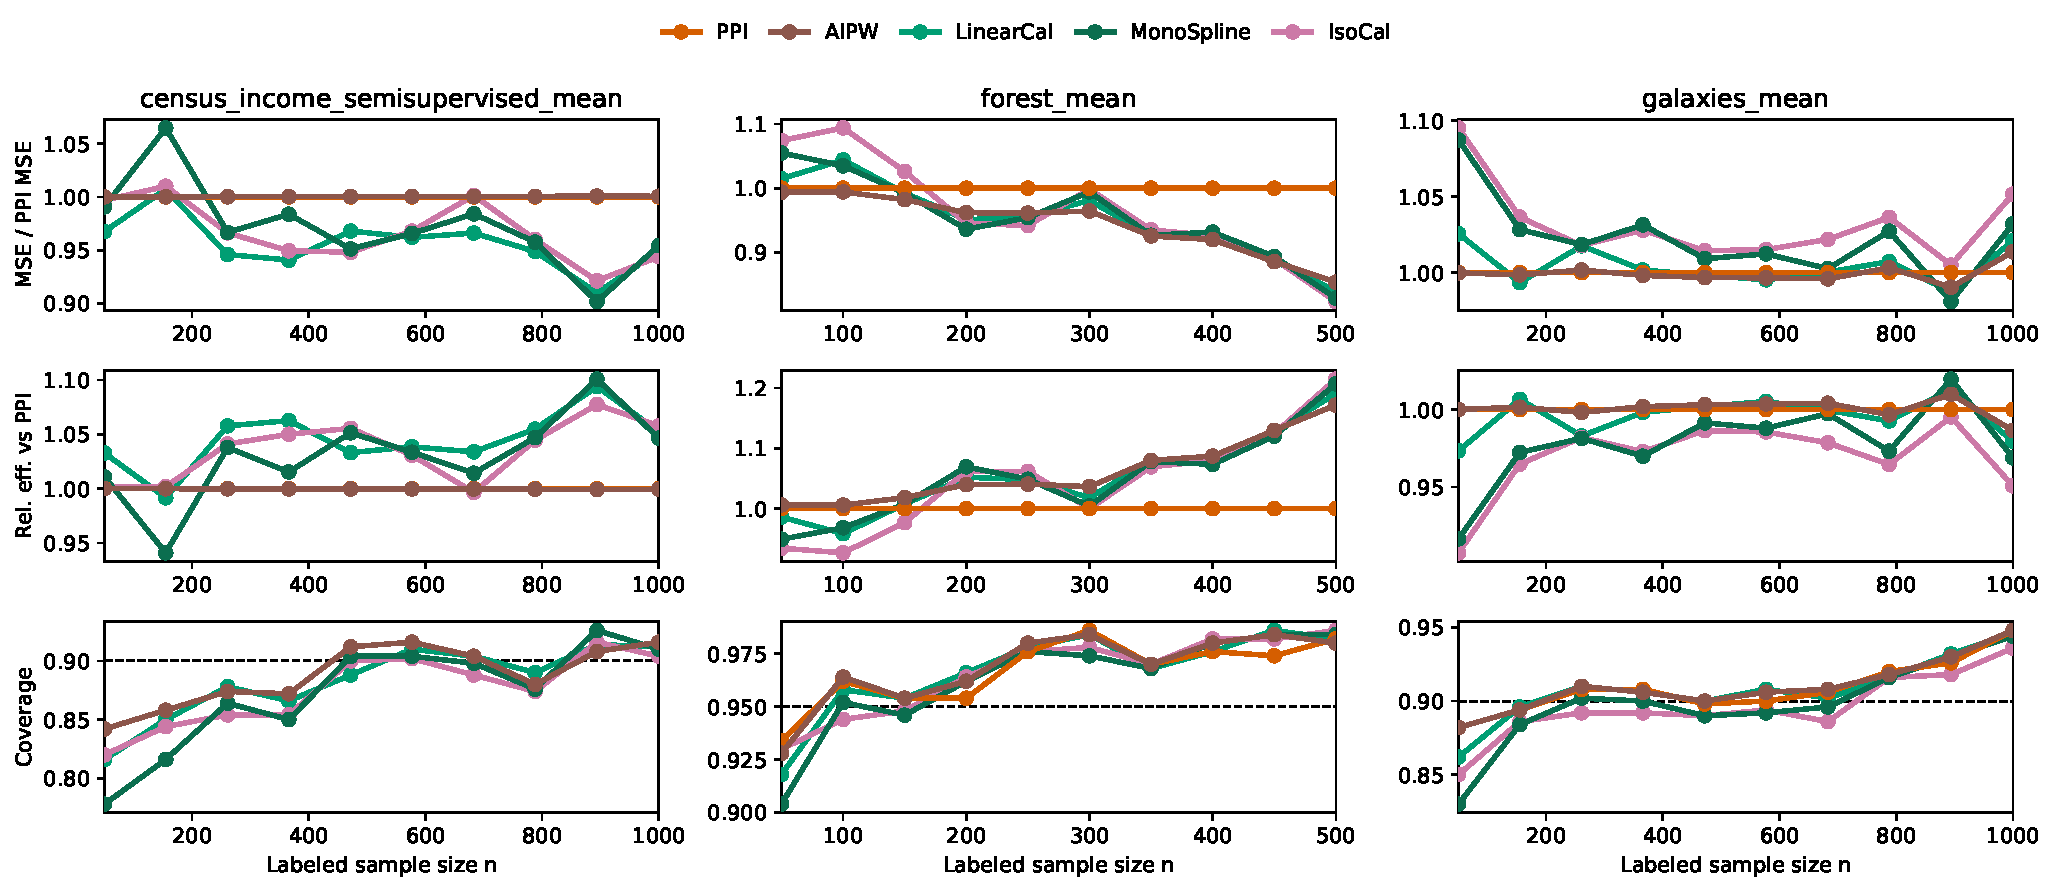
\includegraphics[width=\textwidth]{assets/fig_paper_calibration_grid.pdf}
\caption{Calibration-focused appendix comparison across the reproduced PPI benchmarks, restricted to PPI, AIPW, \texttt{LinearCal}, \texttt{MonoSpline}, and \texttt{IsoCal}. The panels report normalized MSE relative to PPI, relative efficiency versus PPI, and coverage across labeled-sample-size regimes. This figure isolates the fixed-calibration comparison summarized only briefly in the main text for readability.}
\label{fig:ppi-calibration-appendix}
\end{figure}

\begin{figure}[ht]
\centering
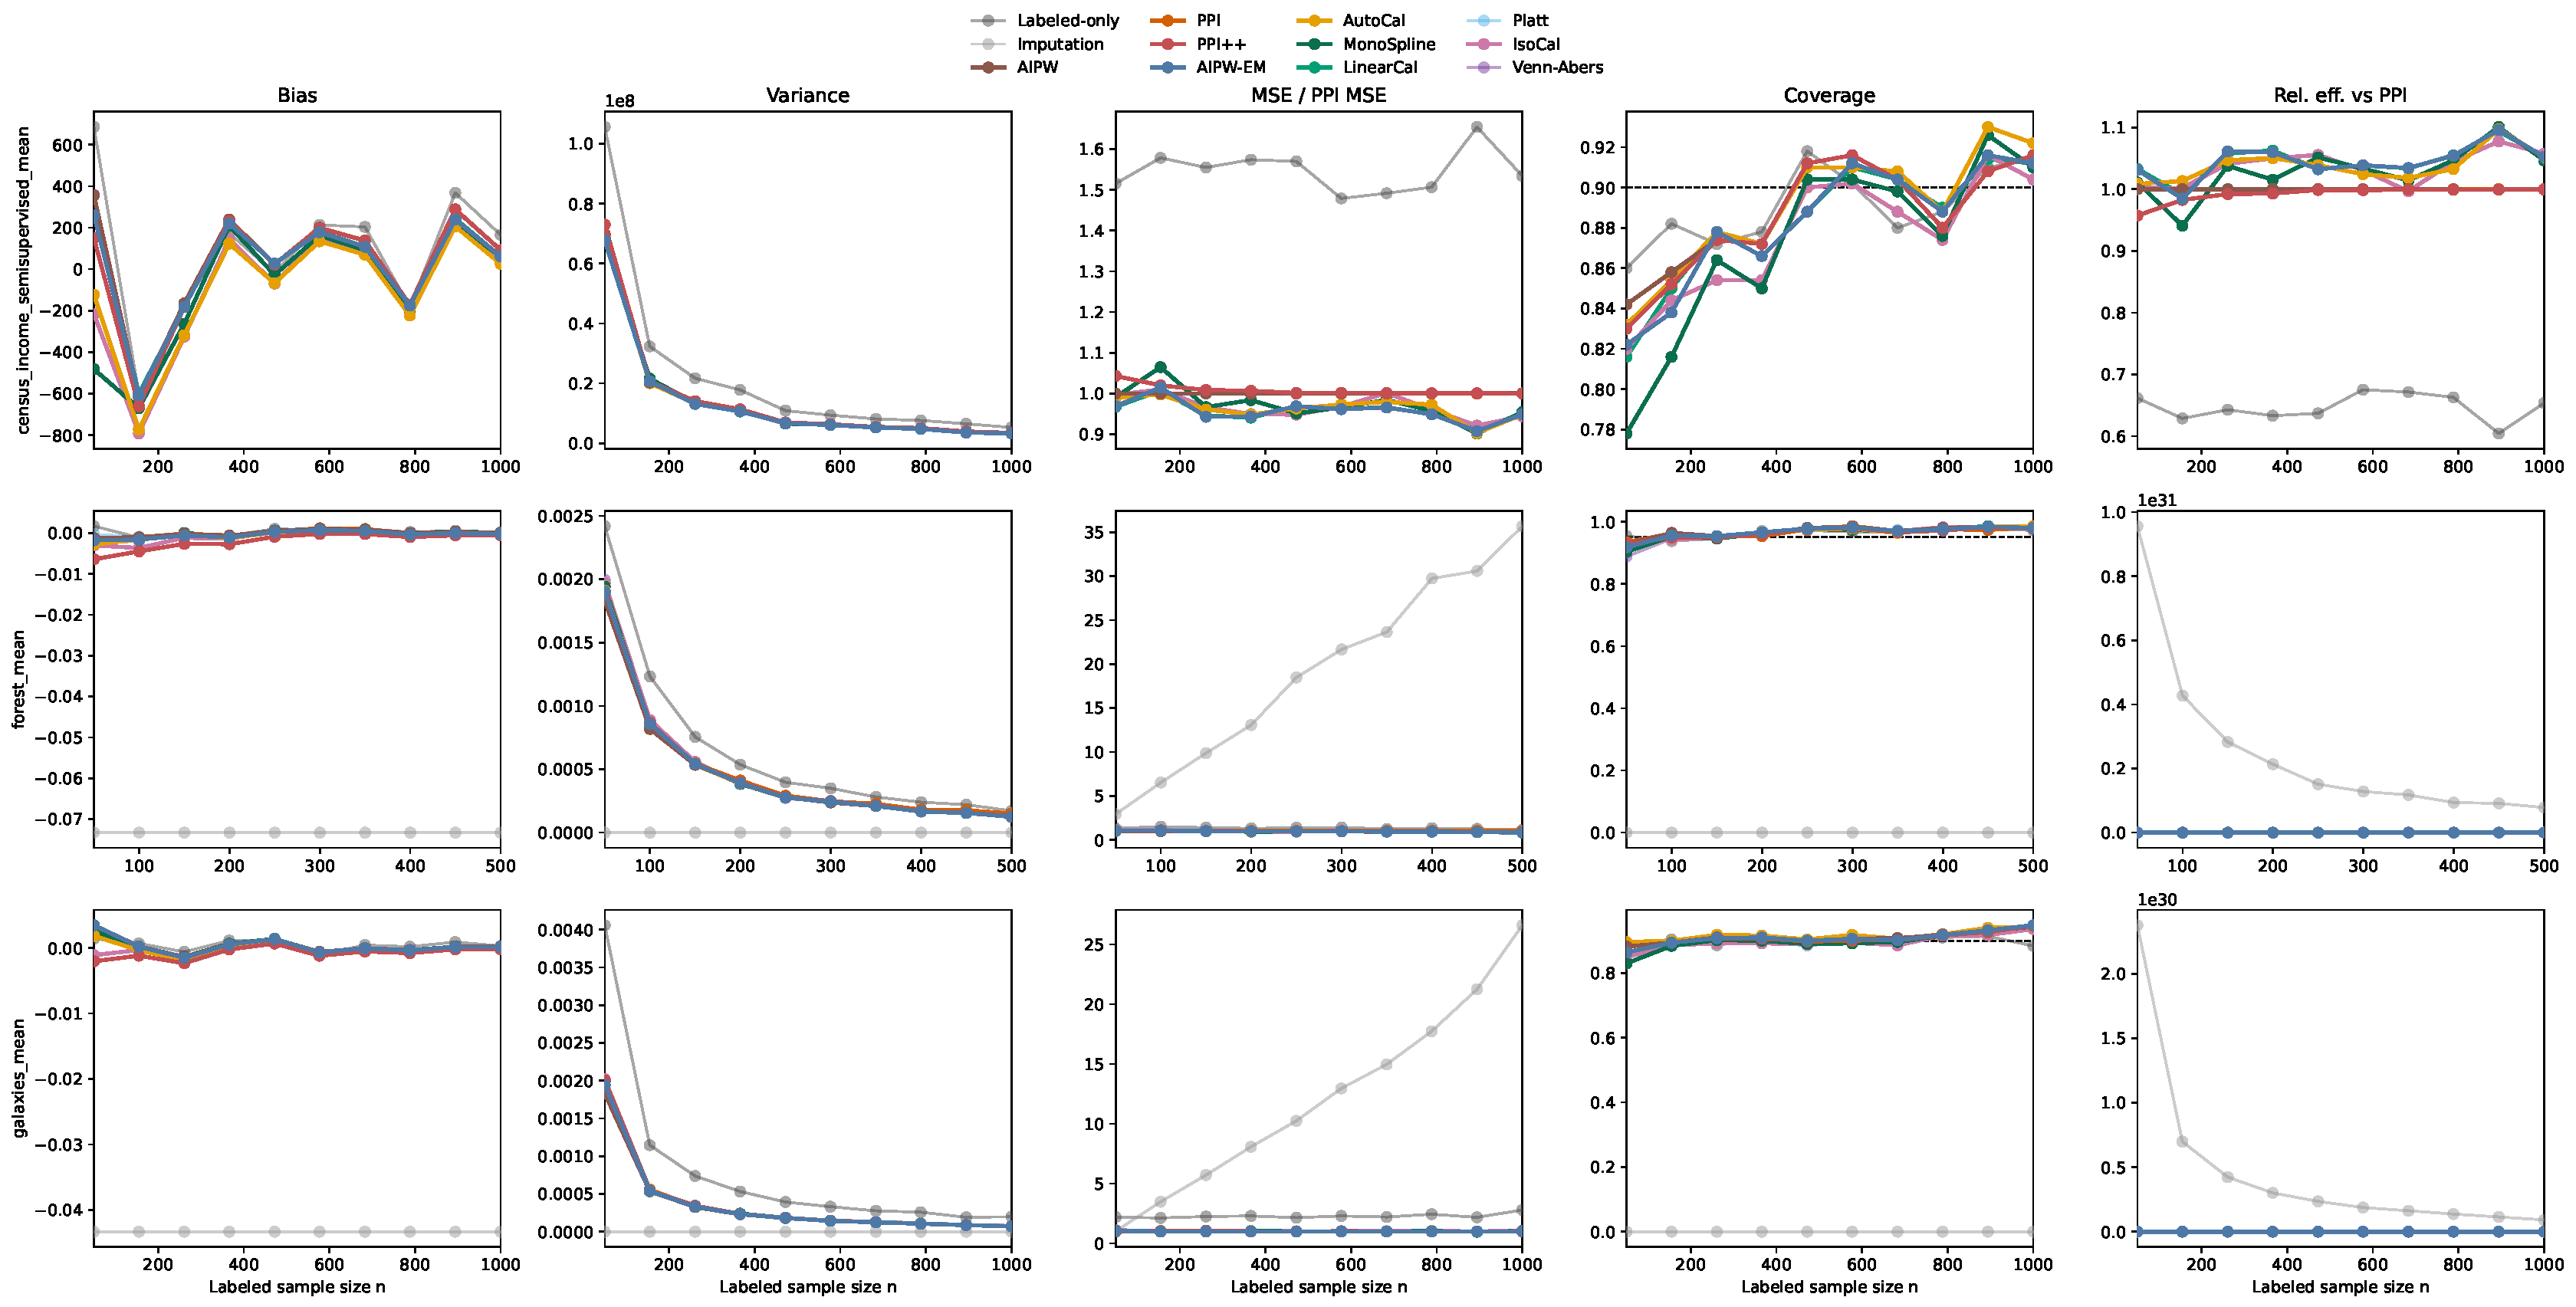
\includegraphics[width=\textwidth]{assets/fig_paper_metric_grid.pdf}
\caption{Full diagnostic grid for the reproduced PPI benchmarks, showing bias, empirical variance, normalized MSE relative to PPI, coverage, and relative efficiency versus PPI across labeled-sample-size regimes. In the normalized-MSE and relative-efficiency panels, the dashed horizontal line marks parity with PPI; in the coverage panels it marks the nominal target coverage \(1-\alpha\). \texttt{AutoCal}, \texttt{MonoSpline}, and \texttt{IsoCal} appear alongside PPI, AIPW, PPI++, \textsc{AIPW-EM}, and the fixed calibration rules, while Platt scaling and Venn--Abers appear only on the binary-outcome datasets where they are well defined.}
\label{fig:ppi-benchmarks-full}
\end{figure}

\subsection{LLM evaluator breakdown}
\label{app:llm-eval-by-evaluator}

The largest raw-score MSE inflation occurs for Skywork and Athene.
The other evaluator summaries show smaller differences among the main-text
estimators. The evaluator-specific results show where calibration provides
the largest gains.

\IfFileExists{assets/table_llm_summary_appendix.tex}{
\begin{table}[ht]
\centering
\small
\resizebox{\textwidth}{!}{\begin{tabular}{lllccc}
\toprule
Track & $n$ & Estimator & MSE / PPI & Label savings & Coverage \\
\midrule
PPE Correctness & 100 & Labeled-only & 0.346 & 0.000 & 0.927 \\
PPE Correctness & 100 & PPI & 1.000 & 0.010 & 0.904 \\
PPE Correctness & 100 & AIPW & 0.774 & 0.009 & 0.906 \\
PPE Correctness & 100 & PPI++ & 0.330 & 0.070 & 0.929 \\
PPE Correctness & 100 & AIPW-EM & 0.309 & 0.095 & 0.930 \\
PPE Correctness & 100 & LinearCal & 0.305 & 0.101 & 0.931 \\
PPE Correctness & 100 & AutoCal & 0.310 & 0.094 & 0.929 \\
PPE Correctness & 100 & MonoSpline & 0.309 & 0.092 & 0.926 \\
PPE Correctness & 100 & IsoCal & 0.309 & 0.089 & 0.925 \\
PPE Correctness & 100 & Platt & 0.304 & 0.102 & 0.930 \\
PPE Correctness & 400 & Labeled-only & 0.299 & 0.000 & 0.988 \\
PPE Correctness & 400 & PPI & 1.000 & 0.020 & 0.924 \\
PPE Correctness & 400 & AIPW & 0.405 & 0.009 & 0.941 \\
PPE Correctness & 400 & PPI++ & 0.276 & 0.083 & 0.989 \\
PPE Correctness & 400 & AIPW-EM & 0.262 & 0.103 & 0.989 \\
PPE Correctness & 400 & LinearCal & 0.260 & 0.105 & 0.989 \\
PPE Correctness & 400 & AutoCal & 0.263 & 0.102 & 0.988 \\
PPE Correctness & 400 & MonoSpline & 0.263 & 0.094 & 0.989 \\
PPE Correctness & 400 & IsoCal & 0.265 & 0.089 & 0.989 \\
PPE Correctness & 400 & Platt & 0.260 & 0.105 & 0.989 \\
PPE Human Preference & 100 & Labeled-only & 0.303 & 0.000 & 0.911 \\
PPE Human Preference & 100 & PPI & 1.000 & 0.004 & 0.897 \\
PPE Human Preference & 100 & AIPW & 0.919 & 0.004 & 0.896 \\
PPE Human Preference & 100 & PPI++ & 0.298 & 0.027 & 0.912 \\
PPE Human Preference & 100 & AIPW-EM & 0.295 & 0.031 & 0.909 \\
PPE Human Preference & 100 & LinearCal & 0.295 & 0.031 & 0.909 \\
PPE Human Preference & 100 & AutoCal & 0.297 & 0.028 & 0.908 \\
PPE Human Preference & 100 & MonoSpline & 0.297 & 0.025 & 0.903 \\
PPE Human Preference & 100 & IsoCal & 0.297 & 0.024 & 0.905 \\
PPE Human Preference & 400 & Labeled-only & 0.289 & 0.000 & 0.945 \\
PPE Human Preference & 400 & PPI & 1.000 & 0.005 & 0.915 \\
PPE Human Preference & 400 & AIPW & 0.703 & 0.004 & 0.917 \\
PPE Human Preference & 400 & PPI++ & 0.283 & 0.025 & 0.946 \\
PPE Human Preference & 400 & AIPW-EM & 0.282 & 0.028 & 0.945 \\
PPE Human Preference & 400 & LinearCal & 0.282 & 0.028 & 0.944 \\
PPE Human Preference & 400 & AutoCal & 0.282 & 0.027 & 0.944 \\
PPE Human Preference & 400 & MonoSpline & 0.282 & 0.027 & 0.942 \\
PPE Human Preference & 400 & IsoCal & 0.282 & 0.026 & 0.940 \\
\bottomrule
\end{tabular}
}
\caption{Appendix PPE-only numerical summary at \(n\in\{100,400\}\), expanding the main-text table to include the efficiency-maximized and additional fixed-calibration comparators omitted there for readability.}
\label{tab:llm-eval-summary-full}
\end{table}
}{}

\IfFileExists{assets/fig_llm_eval_by_evaluator.pdf}{
\begin{figure}[ht]
\centering
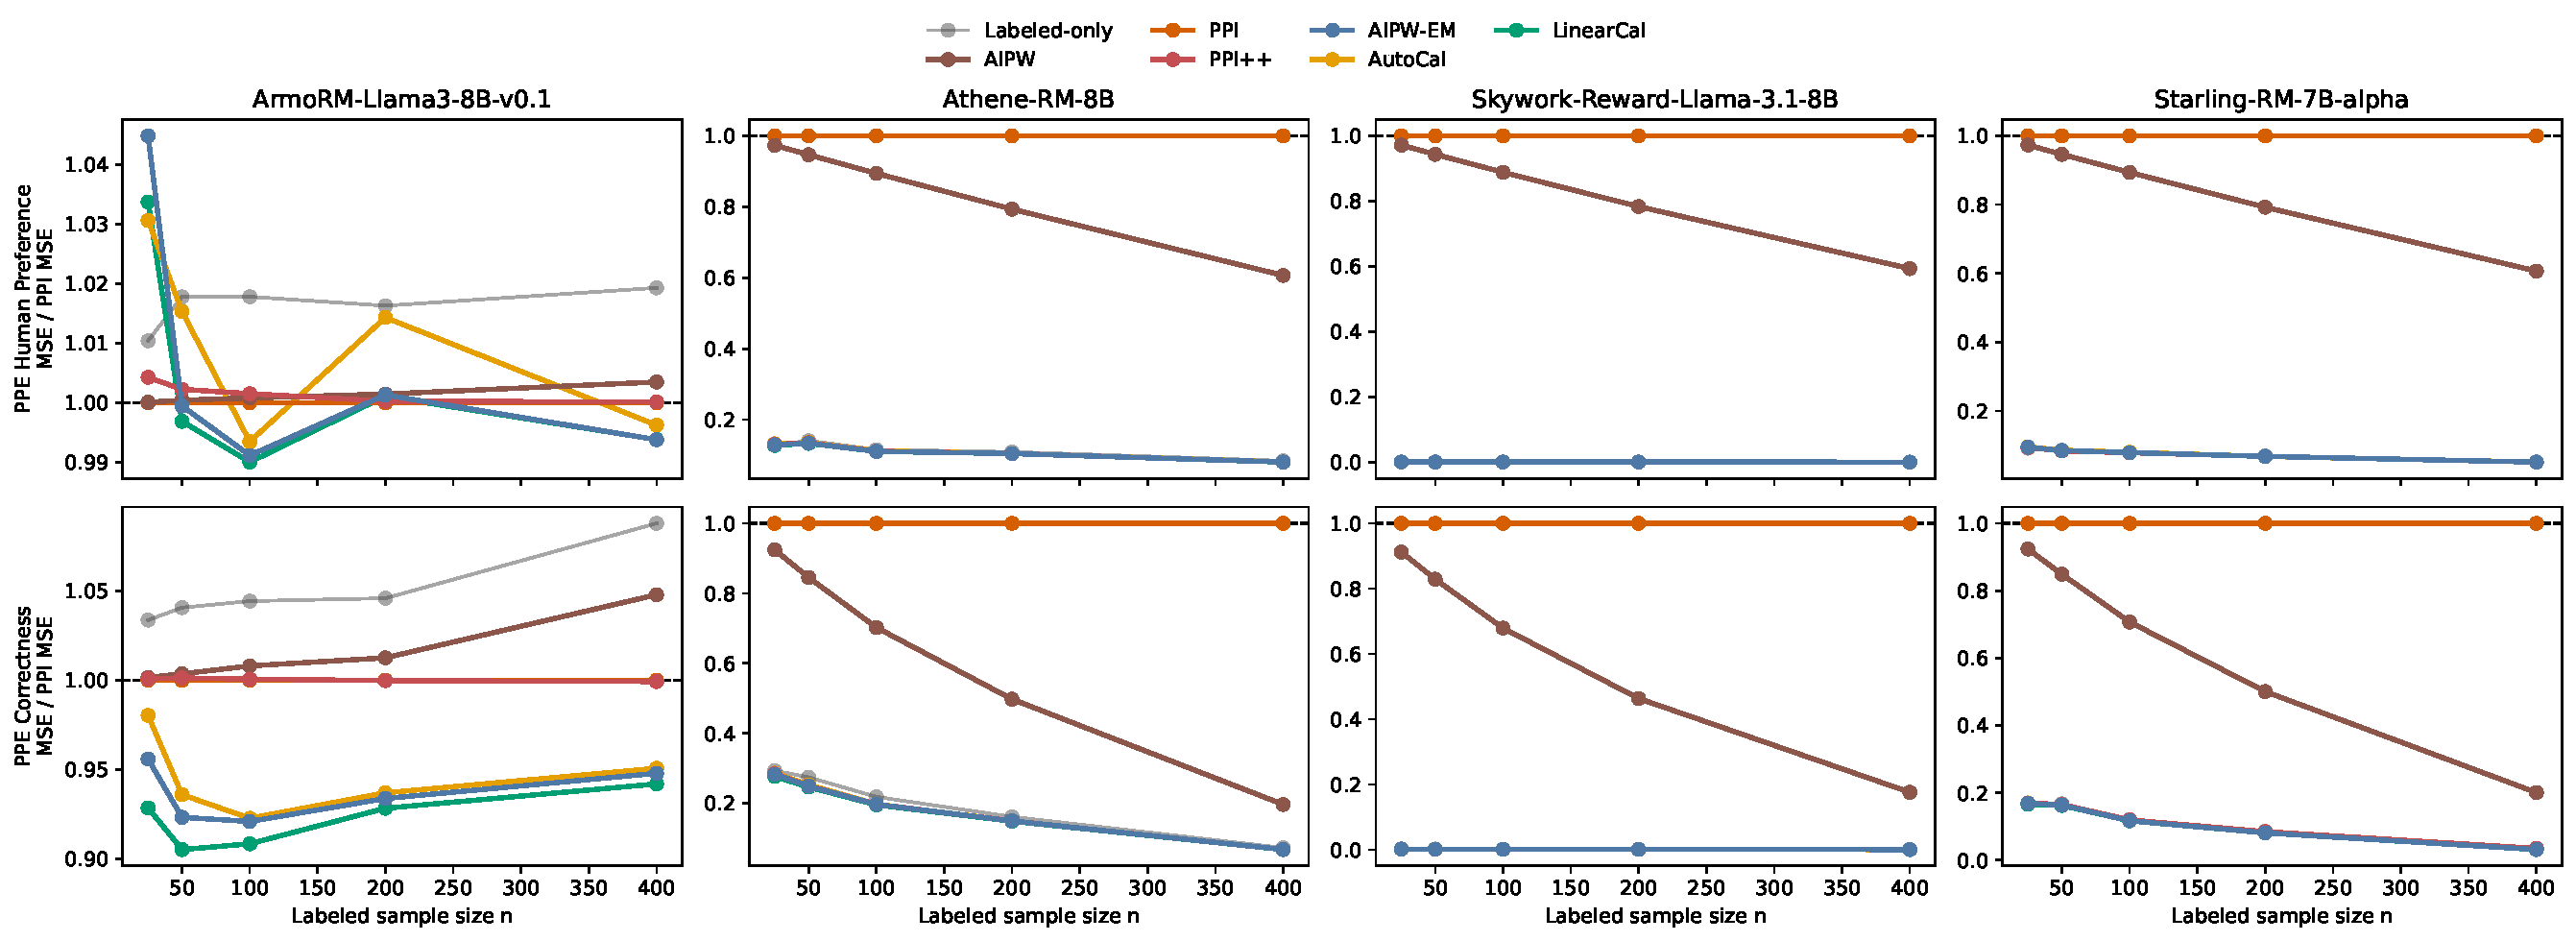
\includegraphics[width=\textwidth]{assets/fig_llm_eval_by_evaluator.pdf}
\caption{Appendix evaluator-specific PPE summary. Each panel repeats the PPE Human and PPE Correctness comparisons for one public evaluator. The large raw-proxy failures are concentrated in Skywork and Athene, while the other evaluator summaries are more benign.}
\label{fig:llm-eval-by-evaluator}
\end{figure}
}{}

\subsection{LLM ranking supplement}
\label{app:llm-ranking}
The PPE human-preference track also induces a downstream ranking problem across the selected target models. Using the same repeated labeled/unlabeled splits as in \cref{sec:llm-benchmark}, we therefore summarize how well each estimator recovers the target-model ordering induced by the full-data human win shares. For each evaluator, labeled-sample size, replicate, and estimator, we rank the eight selected target models by estimated win share, compare that ordering against the ranking induced by the full-data targets, and then macro-average across evaluators. We report Spearman rank correlation, top-1 identification rate, and top-1 regret, defined as the difference in true win share between the best target model and the model selected by the estimator. The main pattern mirrors the mean-estimation results: calibrated and efficiency-maximized estimators substantially outperform raw PPI/AIPW, while remaining close to labeled-only at small \(n\). At \(n=200\), \texttt{AutoCal} attains the highest average Spearman correlation, about \(0.905\); at \(n=400\), \texttt{LinearCal} gives the best overall ranking quality, with Spearman about \(0.941\) and top-1 identification about \(0.646\).

\IfFileExists{assets/table_llm_ppe_ranking.tex}{
\begin{table}[ht]
\centering
\small
\resizebox{0.74\textwidth}{!}{\begin{tabular}{llrrr}
\toprule
$n$ & Estimator & Spearman & Top-1 & Top-1 regret \\
\midrule
25 & AIPW & 0.268 & 0.216 & 0.064 \\
25 & AIPW-EM & 0.599 & 0.344 & 0.028 \\
25 & AutoCal & 0.600 & 0.343 & 0.028 \\
25 & Labeled-only & 0.606 & 0.315 & 0.030 \\
25 & LinearCal & 0.599 & 0.344 & 0.028 \\
25 & PPI & 0.265 & 0.216 & 0.064 \\
25 & PPI++ & 0.594 & 0.336 & 0.029 \\
100 & AIPW & 0.468 & 0.285 & 0.044 \\
100 & AIPW-EM & 0.845 & 0.477 & 0.007 \\
100 & AutoCal & 0.845 & 0.487 & 0.007 \\
100 & Labeled-only & 0.846 & 0.485 & 0.007 \\
100 & LinearCal & 0.846 & 0.482 & 0.007 \\
100 & PPI & 0.456 & 0.279 & 0.046 \\
100 & PPI++ & 0.844 & 0.479 & 0.007 \\
400 & AIPW & 0.631 & 0.439 & 0.027 \\
400 & AIPW-EM & 0.941 & 0.644 & 0.002 \\
400 & AutoCal & 0.941 & 0.640 & 0.002 \\
400 & Labeled-only & 0.940 & 0.625 & 0.002 \\
400 & LinearCal & 0.941 & 0.646 & 0.002 \\
400 & PPI & 0.579 & 0.419 & 0.031 \\
400 & PPI++ & 0.940 & 0.636 & 0.002 \\
\bottomrule
\end{tabular}
}
\caption{Appendix PPE-ranking summary at selected labeled sample sizes from the LLM benchmark. Spearman and top-1 are larger-is-better, while top-1 regret is smaller-is-better.}
\label{tab:llm-ppe-ranking}
\end{table}
}{}

\IfFileExists{assets/fig_llm_ppe_ranking.pdf}{
\begin{figure}[ht]
\centering
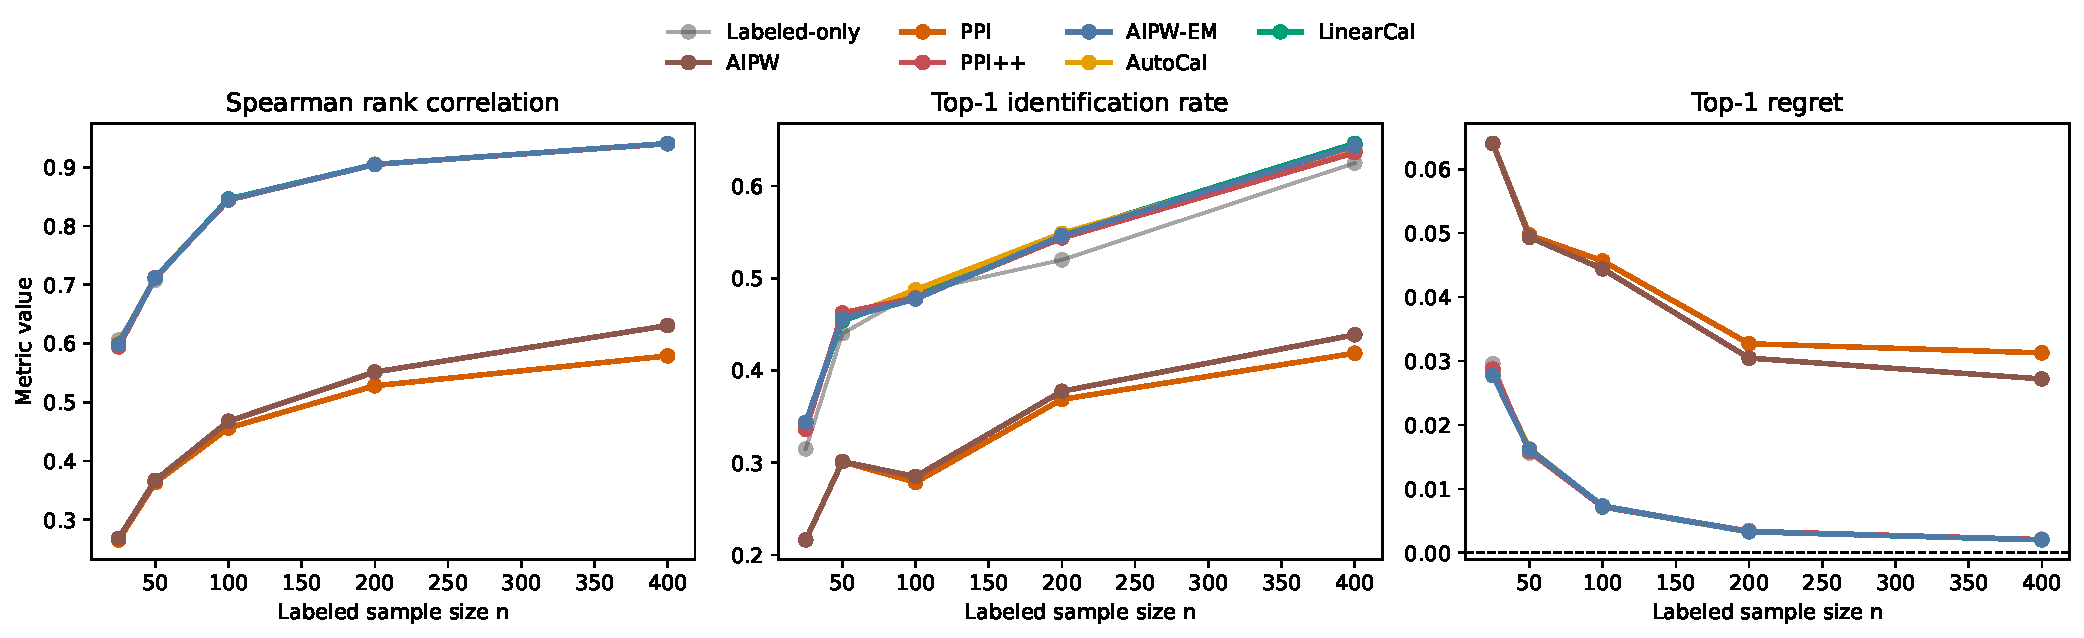
\includegraphics[width=\textwidth]{assets/fig_llm_ppe_ranking.pdf}
\caption{Appendix PPE-ranking supplement from the LLM benchmark, macro-averaged across the public evaluator models. The three panels report Spearman rank correlation, top-1 identification rate, and top-1 regret for recovering the ranking of the eight selected PPE target models from a small labeled sample plus evaluator scores.}
\label{fig:llm-ppe-ranking}
\end{figure}
}{}

\subsection{Data provenance, compute, and reproducibility}
\label{app:compute}

All empirical results use public benchmark sources cited in the main text and appendix. The tabular reproductions use the official \texttt{ppi\_py} mean-estimation datasets; the LLM experiments use PPE Human Preference V1 and PPE correctness data derived from MMLU-Pro, MATH, GPQA, IFEval, and MBPP+. The submission does not introduce a new dataset or foundation model. Figures and tables are generated from the experiment scripts and cached CSV summaries; raw public data and evaluator-score sources remain governed by their upstream licenses and terms.

The main synthetic simulation figure was generated with 2,000 Monte Carlo repetitions per setting. The reproduced PPI benchmark refresh uses 500 random labeled/unlabeled splits for each dataset-size cell. The final PPE run uses 200 rerandomized splits per stage and completed all 112 evaluator/benchmark/target stages. PPE evaluator scores were read from cached or precomputed public score files, so the final aggregation did not run new reward-model inference.

The local runs used Python 3.9.6 with \texttt{numpy} 2.0.2, \texttt{pandas} 2.3.3, \texttt{scikit-learn} 1.6.1, \texttt{xgboost} 2.1.4, \texttt{lightgbm} 4.6.0, \texttt{matplotlib} 3.9.4, and \texttt{ppi-python} 0.2.3. The longest recorded run was the 2,000-repetition main-text simulation sweep, which took about 27,577 seconds on an Apple M1 Pro machine with 10 logical CPUs and 16 GB RAM. The smaller all-comparator simulation refresh took about 1,318 seconds on the same machine.

\section{Anonymous implementation sketch}
\label{appendix:code}

Reference implementations are in \texttt{examples/paper\_calibration.py} in the
supplementary code. The algorithms below use the notation of the paper.

\subsection{Algorithmic summaries}

\begin{algorithm}[t]
\caption{Isotonic-calibrated PPI}
\label{alg:isoppi}
\begin{algorithmic}[1]
\Require \(\mathcal D_L=\{(X_i,Y_i)\}_{i=1}^n\), \(\mathcal D_U=\{\widetilde X_j\}_{j=1}^N\), score \(\mhat\), level \(1-\alpha\)
\State Compute \(T_i=\mhat(X_i)\) and \(\widetilde T_j=\mhat(\widetilde X_j)\)
\State Fit \(\hat f\in\arg\min_{f\in\mathcal F_{\mathrm{iso}}}\sum_{i=1}^n\{Y_i-f(T_i)\}^2\)
\State Set \(q_n^{\mathrm{iso}}(X_i)=\hat f(T_i)\) and \(q_n^{\mathrm{iso}}(\widetilde X_j)=\hat f(\widetilde T_j)\)
\State Form \(\widehat\psi_{\mathrm{iso}}\gets (n+N)^{-1}\{\sum_{i=1}^n q_n^{\mathrm{iso}}(X_i)+\sum_{j=1}^N q_n^{\mathrm{iso}}(\widetilde X_j)\}\)
\State Set \(\widehat D_i^L=q_n^{\mathrm{iso}}(X_i)-\widehat\psi_{\mathrm{iso}}+\rhon^{-1}\{Y_i-q_n^{\mathrm{iso}}(X_i)\}\) and \(\widehat D_j^U=q_n^{\mathrm{iso}}(\widetilde X_j)-\widehat\psi_{\mathrm{iso}}\)
\State Set \(\overline D_L=n^{-1}\sum_{i=1}^n\widehat D_i^L\) and \(\overline D_U=N^{-1}\sum_{j=1}^N\widehat D_j^U\)
\State Set \(\widehat{\mathrm{SE}}_{\mathrm{iso}}^2=(n+N)^{-2}\{\sum_{i=1}^n(\widehat D_i^L-\overline D_L)^2+\sum_{j=1}^N(\widehat D_j^U-\overline D_U)^2\}\)
\State Return \(\widehat\psi_{\mathrm{iso}} \pm z_{1-\alpha/2}\widehat{\mathrm{SE}}_{\mathrm{iso}}\)
\end{algorithmic}
\end{algorithm}

\begin{algorithm}[t]
\caption{Linearly calibrated PPI}
\label{alg:linearppi-basic}
\begin{algorithmic}[1]
\Require \(\mathcal D_L=\{(X_i,Y_i)\}_{i=1}^n\), \(\mathcal D_U=\{\widetilde X_j\}_{j=1}^N\), score \(\mhat\), level \(1-\alpha\)
\State Compute \(T_i=\mhat(X_i)\) and \(\widetilde T_j=\mhat(\widetilde X_j)\)
\State Fit \((\hat a,\hat b)\in\arg\min_{a,b}\sum_{i=1}^n\{Y_i-(aT_i+b)\}^2\)
\State Set \(q_n^{\mathrm{lin}}(X_i)=\hat aT_i+\hat b\) and \(q_n^{\mathrm{lin}}(\widetilde X_j)=\hat a\widetilde T_j+\hat b\)
\State Form \(\widehat\psi_{\mathrm{lin}}\gets (n+N)^{-1}\{\sum_{i=1}^n q_n^{\mathrm{lin}}(X_i)+\sum_{j=1}^N q_n^{\mathrm{lin}}(\widetilde X_j)\}\)
\State Set \(\widehat D_i^L=q_n^{\mathrm{lin}}(X_i)-\widehat\psi_{\mathrm{lin}}+\rhon^{-1}\{Y_i-q_n^{\mathrm{lin}}(X_i)\}\) and \(\widehat D_j^U=q_n^{\mathrm{lin}}(\widetilde X_j)-\widehat\psi_{\mathrm{lin}}\)
\State Set \(\overline D_L=n^{-1}\sum_{i=1}^n\widehat D_i^L\) and \(\overline D_U=N^{-1}\sum_{j=1}^N\widehat D_j^U\)
\State Set \(\widehat{\mathrm{SE}}_{\mathrm{lin}}^2=(n+N)^{-2}\{\sum_{i=1}^n(\widehat D_i^L-\overline D_L)^2+\sum_{j=1}^N(\widehat D_j^U-\overline D_U)^2\}\)
\State Return \(\widehat\psi_{\mathrm{lin}} \pm z_{1-\alpha/2}\widehat{\mathrm{SE}}_{\mathrm{lin}}\)
\end{algorithmic}
\end{algorithm}

\begin{algorithm}[t]
\caption{Linearly calibrated PPI with covariate adjustment}
\label{alg:linearppi}
\begin{algorithmic}[1]
\Require \(\mathcal D_L=\{(X_i,Y_i)\}_{i=1}^n\), \(\mathcal D_U=\{\widetilde X_j\}_{j=1}^N\), score \(\mhat\), level \(1-\alpha\)
\State Compute \(T_i=\mhat(X_i)\) and \(\widetilde T_j=\mhat(\widetilde X_j)\)
\State Fit \((\hat a,\hat\beta,\hat b)\in\arg\min_{a,\beta,b}\sum_{i=1}^n\{Y_i-(a+X_i^\top\beta+bT_i)\}^2\)
\State Set \(q_n^{\mathrm{lin}}(X_i)=\hat a+X_i^\top\hat\beta+\hat bT_i\) and \(q_n^{\mathrm{lin}}(\widetilde X_j)=\hat a+\widetilde X_j^\top\hat\beta+\hat b\widetilde T_j\)
\State Form \(\widehat\psi_{\mathrm{lin}}\gets (n+N)^{-1}\{\sum_{i=1}^n q_n^{\mathrm{lin}}(X_i)+\sum_{j=1}^N q_n^{\mathrm{lin}}(\widetilde X_j)\}\)
\State Set \(\widehat D_i^L=q_n^{\mathrm{lin}}(X_i)-\widehat\psi_{\mathrm{lin}}+\rhon^{-1}\{Y_i-q_n^{\mathrm{lin}}(X_i)\}\) and \(\widehat D_j^U=q_n^{\mathrm{lin}}(\widetilde X_j)-\widehat\psi_{\mathrm{lin}}\)
\State Set \(\overline D_L=n^{-1}\sum_{i=1}^n\widehat D_i^L\) and \(\overline D_U=N^{-1}\sum_{j=1}^N\widehat D_j^U\)
\State Set \(\widehat{\mathrm{SE}}_{\mathrm{lin}}^2=(n+N)^{-2}\{\sum_{i=1}^n(\widehat D_i^L-\overline D_L)^2+\sum_{j=1}^N(\widehat D_j^U-\overline D_U)^2\}\)
\State Return \(\widehat\psi_{\mathrm{lin}} \pm z_{1-\alpha/2}\widehat{\mathrm{SE}}_{\mathrm{lin}}\)
\end{algorithmic}
\end{algorithm}

\clearpage

\section*{NeurIPS Paper Checklist}

\begin{enumerate}[leftmargin=5mm]
\item \textbf{Claims}

Question: Do the main claims made in the abstract and introduction accurately
reflect the paper's contributions and scope?

Answer: \answerYes{}.

Justification: The abstract and introduction state the main claims, and the
paper distinguishes exact representation results, asymptotic theory, and
empirical findings; see \cref{sec:setup,sec:calppi,sec:theory,sec:exp}.

\textbf{Guidelines:}
\begin{itemize}[leftmargin=5mm, noitemsep]
\item The answer should be yes, no, or n/a.
\item Claims in the abstract and introduction should match the paper's
contributions and scope.
\item Important assumptions and limitations should be clearly stated.
\end{itemize}

\item \textbf{Limitations}

Question: Does the paper discuss the limitations of the work performed by the
authors?

Answer: \answerYes{}.

Justification: The conclusion and theory sections state the main scope
limitations: the strongest guarantees use the known-\(\rho_n\) two-sample
design, a fixed or appropriately cross-fitted score, and a stable second-stage
calibrator; see \cref{sec:theory,appendix:remarks}.

\textbf{Guidelines:}
\begin{itemize}[leftmargin=5mm, noitemsep]
\item The answer should be yes, no, or n/a.
\item Authors are encouraged to discuss strong assumptions, robustness to
violations of those assumptions, and the practical scope of the claims.
\item The answer n/a means the paper has no limitations; the answer no means
limitations exist but are not discussed.
\end{itemize}

\item \textbf{Theory assumptions and proofs}

Question: For each theoretical result, does the paper provide the full set of
assumptions and a complete proof?

Answer: \answerYes{}.

Justification: The main assumptions are stated in \cref{sec:setup,sec:theory},
with complete proofs collected in
\cref{app:repr,sec:ppi++,app:eif,app:al,app:eff}.

\textbf{Guidelines:}
\begin{itemize}[leftmargin=5mm, noitemsep]
\item The answer should be yes, no, or n/a.
\item All assumptions should be stated or referenced in theorem and lemma
statements.
\item Complete proofs may appear in the main paper or appendix; informal proof
sketches in the main text should be backed by formal proofs.
\item Theorems, lemmas, and external results used in proofs should be properly
referenced.
\end{itemize}

\item \textbf{Experimental result reproducibility}

Question: If the contribution is a dataset, model, algorithm, or empirical
evaluation, what steps were taken to make the results reproducible or
verifiable?

Answer: \answerYes{}.

Justification: The main experimental takeaways appear in \cref{sec:exp}, with
benchmark construction, additional diagnostics, evaluator-specific LLM results,
ranking results, and compute details in
\cref{app:empirical,app:llm-eval-by-evaluator,app:llm-ranking,app:compute}.

\textbf{Guidelines:}
\begin{itemize}[leftmargin=5mm, noitemsep]
\item The answer should be yes, no, or n/a.
\item Reproducibility can be supported by detailed algorithm descriptions,
instructions, code, data, checkpoints, hosted access, or other appropriate
avenues.
\item If reproducibility is limited, the paper should explain the available
path for verifying or reproducing the main claims.
\end{itemize}

\item \textbf{Open access to data and code}

Question: If the paper includes experiments, does it include the code, data,
and instructions needed to reproduce the main experimental results, either in
the supplemental material or as a URL?

Answer: \answerYes{}.

Justification: The experiments use public benchmark sources cited in the paper,
and the submission includes anonymous implementation sketches and can be
accompanied by an anonymous supplementary artifact. Repository and
project-website links are omitted from the double-blind PDF; see
\cref{appendix:code,app:compute}.

\textbf{Guidelines:}
\begin{itemize}[leftmargin=5mm, noitemsep]
\item The answer should be yes, no, or n/a.
\item Instructions should include the exact commands and environment needed to
reproduce the main experimental results, including the new method and baselines.
\item If only a subset of experiments is reproducible, the paper should say
which subset.
\item At submission time, released links or archives should preserve anonymity.
\end{itemize}

\item \textbf{Experimental setting/details}

Question: If the paper includes experiments, does it specify all training and
test details, including data splits, hyperparameters, and how they were chosen?

Answer: \answerYes{}.

Justification: The simulation design, benchmark protocols, estimator sets,
repetition counts, evaluator sources, and summary metrics are described in
\cref{sec:exp,app:empirical,app:compute}.

\textbf{Guidelines:}
\begin{itemize}[leftmargin=5mm, noitemsep]
\item The answer should be yes, no, or n/a.
\item The answer n/a means the paper does not include experiments.
\item Important experimental details should appear in the main paper; full
details may also appear in the appendix, code, or supplemental material.
\item Hyperparameter choices and selection procedures should be stated.
\end{itemize}

\item \textbf{Experiment statistical significance}

Question: Does the paper report error bars suitably and correctly defined or
other appropriate information about the statistical significance of the
experiments?

Answer: \answerYes{}.

Justification: The experiments report Monte Carlo variability, MSE, interval
coverage, and efficiency comparisons over repeated random splits, and the
inference procedures are tied to the Wald theory in \cref{sec:theory}; see also
\cref{cor:normal}.

\textbf{Guidelines:}
\begin{itemize}[leftmargin=5mm, noitemsep]
\item The answer should be yes, no, or n/a.
\item The answer n/a means the paper does not include experiments.
\item Error bars, confidence intervals, or significance tests should be
reported for experiments supporting the main claims when appropriate.
\item The paper should state what source of variability is shown and how error
bars or intervals are computed.
\end{itemize}

\item \textbf{Experiments compute resources}

Question: For each experiment, does the paper provide sufficient information on
the computer resources needed to reproduce the experiments?

Answer: \answerYes{}.

Justification: Hardware, major software versions, repetition counts, cache
usage, completed LLM stages, and recorded wall-clock times are reported in
\cref{app:compute}.

\textbf{Guidelines:}
\begin{itemize}[leftmargin=5mm, noitemsep]
\item The answer should be yes, no, or n/a.
\item The answer n/a means the paper does not include experiments.
\item The paper should describe the compute type, memory or hardware when
relevant, per-run compute, and estimated total compute.
\item The paper should disclose whether substantially more compute was used for
the project than for the reported experiments.
\end{itemize}

\item \textbf{Code of ethics}

Question: Have the authors read the NeurIPS Code of Ethics and ensured that the
research conforms to it?

Answer: \answerYes{}.

Justification: The paper is a methodological contribution in semisupervised
statistical inference, and we are not aware of any aspect of the work that
conflicts with the NeurIPS Code of Ethics.

\textbf{Guidelines:}
\begin{itemize}[leftmargin=5mm, noitemsep]
\item The answer should be yes or no, with explanation if needed.
\item Any special circumstances requiring deviation from the NeurIPS Code of
Ethics should be explained while preserving anonymity.
\end{itemize}

\item \textbf{Broader impacts}

Question: If appropriate for the scope and focus of the paper, does it discuss
potential negative societal impacts of the work performed?

Answer: \answerNA{}.

Justification: The paper develops estimation and inference methodology rather
than a deployed decision system, though misuse of semisupervised estimators in
high-stakes applications remains a general concern.

\textbf{Guidelines:}
\begin{itemize}[leftmargin=5mm, noitemsep]
\item The answer should be yes, no, or n/a.
\item Authors should discuss plausible negative impacts when there is a direct
path to misuse, fairness, privacy, security, or other societal harms.
\item Foundational or generic methods may answer n/a when no direct negative
application is apparent, but limitations and deployment risks should still be
handled honestly.
\item Mitigations may be discussed when negative impacts are identified.
\end{itemize}

\item \textbf{Safeguards}

Question: Does the paper describe safeguards for responsible release of data or
models that have a high risk for misuse?

Answer: \answerNA{}.

Justification: The paper does not introduce a system that generates content or
interacts with users, and it does not release new high-risk artifacts requiring
special safeguards.

\textbf{Guidelines:}
\begin{itemize}[leftmargin=5mm, noitemsep]
\item The answer should be yes, no, or n/a.
\item High-risk or dual-use model releases should include appropriate access,
usage, or release safeguards.
\item Dataset releases that may contain unsafe content should describe how
unsafe material was avoided or controlled.
\end{itemize}

\item \textbf{Licenses for existing assets}

Question: If existing assets are used, are the creators or original owners
properly credited and are the license and terms of use respected?

Answer: \answerYes{}.

Justification: The paper cites the public benchmark sources and software
ecosystems used in the experiments, does not redistribute new raw datasets in
the PDF, and records data provenance and dependency versions in
\cref{app:compute}. Any anonymous supplement should preserve upstream license
and terms-of-use files where required.

\textbf{Guidelines:}
\begin{itemize}[leftmargin=5mm, noitemsep]
\item The answer should be yes, no, or n/a.
\item Existing code, data, models, and benchmarks should be cited and their
licenses or terms of use should be respected.
\item Versions and URLs should be provided when possible.
\item If releasing derived assets, the original and derived licenses should be
stated where applicable.
\end{itemize}

\item \textbf{New assets}

Question: If new assets are released, are they documented and are relevant
details provided alongside the assets?

Answer: \answerNA{}.

Justification: The paper does not introduce a new dataset, benchmark, or
foundation model; generated figures and tables are derived from cited public
benchmarks.

\textbf{Guidelines:}
\begin{itemize}[leftmargin=5mm, noitemsep]
\item The answer should be yes, no, or n/a.
\item The answer n/a means the paper does not release new assets.
\item New datasets, code, or models should be documented with training,
license, limitations, and intended-use details as relevant.
\item Released assets should be anonymized for initial submission when
applicable.
\end{itemize}

\item \textbf{Crowdsourcing and research with human subjects}

Question: For crowdsourcing experiments and research with human subjects, does
the paper include the full text of instructions given to participants and
screenshots, if applicable, as well as details about compensation (if any)?

Answer: \answerNA{}.

Justification: The paper analyzes existing public benchmark labels and does not
conduct new human-subject experiments or crowdsourcing.

\textbf{Guidelines:}
\begin{itemize}[leftmargin=5mm, noitemsep]
\item The answer should be yes, no, or n/a.
\item The full participant instructions, screenshots, and compensation details
should be included when applicable, with more detail in the main paper when
human subjects are central to the contribution.
\item Work involving data collection, curation, or other labor should follow
the NeurIPS Code of Ethics, including compensation requirements.
\end{itemize}

\item \textbf{Institutional review board (IRB) approvals or equivalent for
research with human subjects}

Question: If human-subject research was conducted, does the paper describe
participant risks and whether IRB or equivalent approval was obtained?

Answer: \answerNA{}.

Justification: The paper uses existing public benchmark data and does not
involve new crowdsourcing or human-subject research.

\textbf{Guidelines:}
\begin{itemize}[leftmargin=5mm, noitemsep]
\item The answer should be yes, no, or n/a.
\item IRB or equivalent review should be described when required by the
relevant institution or jurisdiction.
\item Initial submissions should not include information that breaks anonymity,
such as the reviewing institution, when applicable.
\end{itemize}

\item \textbf{Declaration of LLM usage}

Question: Does the paper describe the usage of LLMs if it is an important,
original, or non-standard component of the core methods in this research?

Answer: \answerYes{}.

Justification: LLMs enter only through the empirical LLM-evaluation benchmark,
where public precomputed evaluator-score sources and PPE datasets are described
in \cref{sec:exp,app:llm-eval-by-evaluator,app:llm-ranking,app:compute}; they
are not an important, original, or non-standard component of the proposed
methodology.

\textbf{Guidelines:}
\begin{itemize}[leftmargin=5mm, noitemsep]
\item The answer should be yes, no, or n/a.
\item The paper should describe LLM use that is important, original, or
non-standard for the core method, experiments, evaluation, or data generation.
\item The answer n/a means LLMs are not important, original, or non-standard
components of the core method.
\item LLM use only for writing, editing, or formatting does not need to be
declared when it does not affect methodology, rigor, or originality.
\end{itemize}
\end{enumerate}

\end{document}
